%\documentclass[handout,xcolor=pdftex,dvipsnames,table,mathserif]{beamer}
\documentclass[xcolor=pdftex,dvipsnames,table,mathserif]{beamer}
%\usepackage{subfigure}
\usepackage{amsbsy}
\usepackage{tikz}
\usetikzlibrary{arrows}
\usepackage{amsmath,graphicx,dsfont,color}
\usepackage{amsfonts}
\usepackage{amssymb}
\usepackage{array}

\usepackage{subfig}

% makes the subfig package work
\makeatletter
\let\@@magyar@captionfix\relax
\makeatother

% subfigure counter resets every frame
\makeatletter
\@addtoreset{subfigure}{framenumber}
\makeatother

% First author and year
\bibliographystyle{apalike}

% This sets the list items of the bibliography to the same symbol used for citation.
\setbeamertemplate{bibliography item}{\insertbiblabel}

% This avoids extralines for different entries
\setbeamertemplate{bibliography entry title}{}
\setbeamertemplate{bibliography entry location}{}
\setbeamertemplate{bibliography entry note}{}

\DeclareMathOperator*{\argmin}{arg\,min}
\DeclareMathOperator*{\argmax}{arg\,max}
%Definitiona

\newcommand{\x}{\mathbf{x}}
\newcommand{\X}{\mathbf{X}}
\newcommand{\W}{\mathbf{W}} %Weight
\newcommand{\bais}{\mathbf{b}}%Bais
\newcommand{\act}{\texttt{g}}%Activation
\newcommand{\loss}{L}
\newcommand{\pdata}{\hat{p}_{\texttt{data}}}
\newcommand{\nsize}{N}
\newcommand{\nfeatures}{P}
\newcommand{\param}{\boldsymbol{\theta}}
\newcommand{\featmap}{\boldsymbol{\phi}}
\newcommand{\EV}{\mathbb{E}}







\usepackage{physics}

\graphicspath{{../graphics/}}

\AtBeginSection[]{
  \begin{frame}{Contents}
    \tableofcontents[currentsection, hideothersubsections]
  \end{frame}
}

\AtBeginSubsection[]{
  \begin{frame}{Contents}
    \tableofcontents[currentsection, subsectionstyle=show/shaded/hide]
  \end{frame}
}

\setbeamertemplate{footline}[frame number]{}
\setbeamertemplate{navigation symbols}{}
\setbeamertemplate{section in toc}[square]
\setbeamertemplate{items}[square]

\newcommand{\myvec}[1]{\ensuremath{\begin{pmatrix}#1\end{pmatrix}}}

%% For image credits on image bottom right
\usepackage[absolute,overlay]{textpos}
\setbeamercolor{framesource}{fg=gray}
\setbeamerfont{framesource}{size=\tiny}
\newcommand{\source}[1]{\begin{textblock*}{4cm}(8.7cm,8.6cm)
    \begin{beamercolorbox}[ht=0.5cm,right]{framesource}
      \usebeamerfont{framesource}\usebeamercolor[fg]{framesource} Credits: {#1}
    \end{beamercolorbox}
\end{textblock*}}

%%%%%%%%%%%%%%%%%%%%%%%%%%%%%%%%%%%%
%% \begin{frame}{Quizz}

%%   \begin{block}{Question}
%%   \begin{itemize}
%%   \item[A/]
%%   \item[B/]
%%   \item[C/]
%%   \item[D/]
%%   \end{itemize}

%%   \end{block}

%% \end{frame}


%% édition
%% (pas de mot de passe) / lien vers l'éditeur de quiz
%% http://www.quizzoodle.com/quizz/editor/9191b836f17f443a997bcbe08755b2de

%% session
%% (pas de mot de passe) / lien vers le gestionnaire de sessions
%% http://www.quizzoodle.com/session/1be8ffbacabd4a7d9109772cc24d4d8e

%% supprimer
%% mdp: delete / lien pour supprimer le quiz
%% http://www.quizzoodle.com/quizz/delete/5c19c98d6bb54bbabfaf042caffca39e

\title{Convolutional neural networks}
\author{E. Decencière}
\date{MINES ParisTech\\
  PSL Research University\\
  Center for Mathematical Morphology
}
\titlegraphic{
\includegraphics[height=1.7cm]{../graphics/logoemp}}

\useinnertheme{rounded}
\usecolortheme{rose}

%%%%%%%%%%%%%%%%%%%%%%%%%%%%%%%%%%%%%%%%%%%%%%%%%%
%%%%%%%%%%%%%%%%%%%%%%%%%%%%%%%%%%%%%%%%%%%%%%%%%%
\begin{document}

\begin{frame}
  \titlepage
\end{frame}

%%%%%%%%%%%%%%%%%%%%%%%%%%%%%%%%%%%%
%% \begin{frame}{Correction TP 1}

%%   \begin{itemize}
%%   \item Utilisation de Google Drive
%%   \item Optimiser le réseau pour les bases Moons et Circles
%%     \begin{itemize}
%%     \item Meilleures valeurs de $q$ et $lr$ ?
%%     \end{itemize}
%%   \item Codage de l'entropie croisée et de sa dérivée. \alert{Attention à la dernière activation!}
%%   \item Comparaison:
%%     \begin{itemize}
%%     \item Besoin d'une base de \alert{test}.
%%     \item Quantification.
%%     \end{itemize}
%%   \end{itemize}

%% \end{frame}

%%%%%%%%%%%%%%%%%%%%%%%%%%%%%%%%%%%%%%%%%%%%%%%%%%
\frame{
  \frametitle{Contents}
  \tableofcontents[hidesubsections]
}


%%%%%%%%%%%%%%%%%%%%%%%%%%%%%%%%%%%%%%%%%%%%%%%%%%
\section{Introduction}
%%%%%%%%%%%%%%%%%%%%%%%%%%%%%%%%%%%%%%%%%%%%%%%%%%

%%%%%%%%%%%%%%%%%%%%%%%%%%%%%%%%%%%%
\begin{frame}{A picture is worth a thousand words}

  \begin{columns}
    \begin{column}{.5\textwidth}
      \begin{block}{Definition}
        \begin{itemize}
        \item Classically, an image is a matrix of values belonging to $[0, \ldots, 255]$ (grey level images) or to $[0, \ldots, 255]^3$ (color images).
        \item More generally, an image is a $q$-dimensional array of values belonging to $R^d$.
        \end{itemize}
      \end{block}

    \end{column}

    \begin{column}{.5\textwidth}
      \begin{figure}
        \centering
        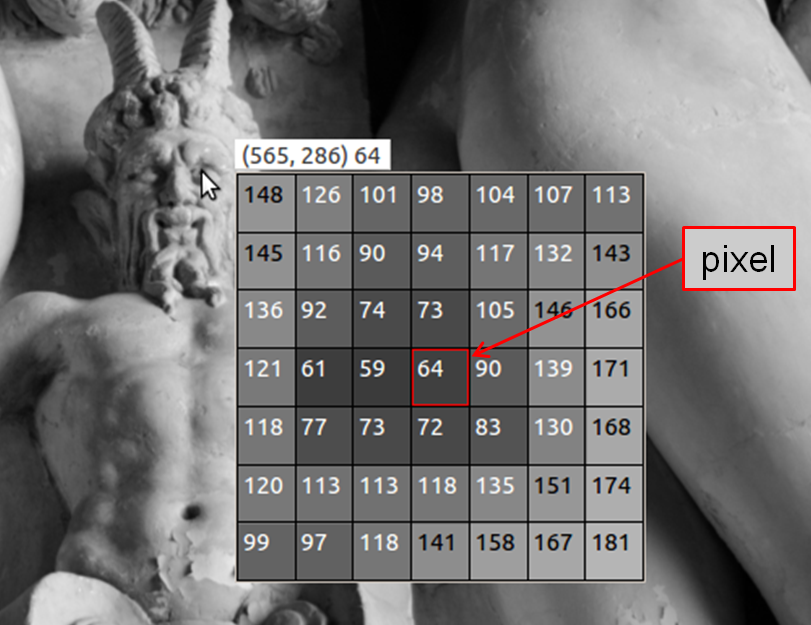
\includegraphics[width=5cm]{../graphics/faune.png}\\
        \tiny{Grey level values around the left eye of the faun}
      \end{figure}

    \end{column}
  \end{columns}

  \pause

  \begin{block}{Examples}
    \begin{itemize}
    \item Grey level 2D images: infrared, microscopy, topography
    \item Colour images: camera photos
    \item Grey level 3D images: computed tomography scan
    \item Colour image sequences: video, motion pictures
    \item $d > 3$: multi-spectral imaging
    \end{itemize}
  \end{block}

\end{frame}

%%%%%%%%%%%%%%%%%%%%%%%%%%%%%%%%%%%%
\begin{frame}{What is special about images?}

  \begin{columns}
    \begin{column}{.5\textwidth}
      \begin{figure}[ht]
        \centering
        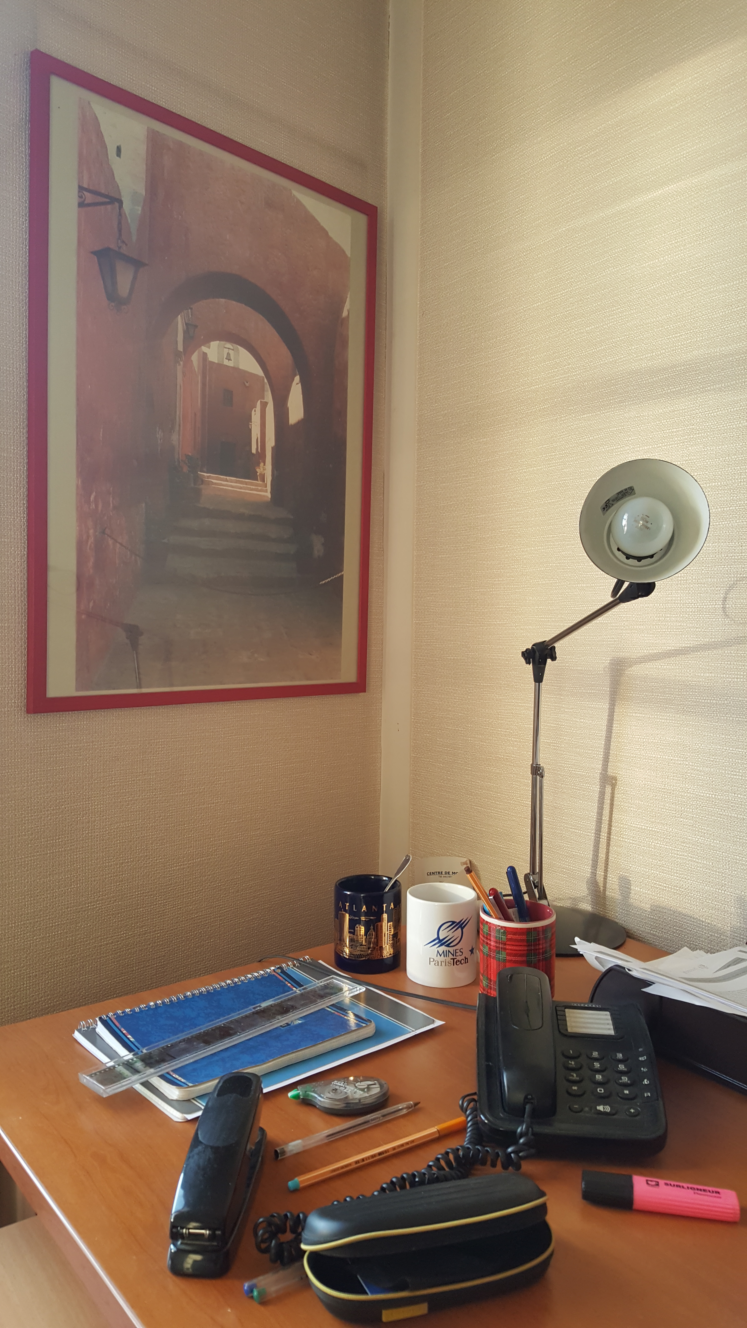
\includegraphics[height=8cm]{bureau-1}
      \end{figure}

    \end{column}
    \begin{column}{.5\textwidth}
      \begin{itemize}
      \item Local structure
      \item Spatial redundancy
      \item Scale redundancy \cite{glasner_super-resolution_2009}
      \end{itemize}
    \end{column}

  \end{columns}

\end{frame}

%%%%%%%%%%%%%%%%%%%%%%%%%%%%%%%%%%%%
\begin{frame}{Extracting semantic information from an image}

  \begin{columns}
    \begin{column}{.5\textwidth}
      \begin{figure}[ht]
        \centering
        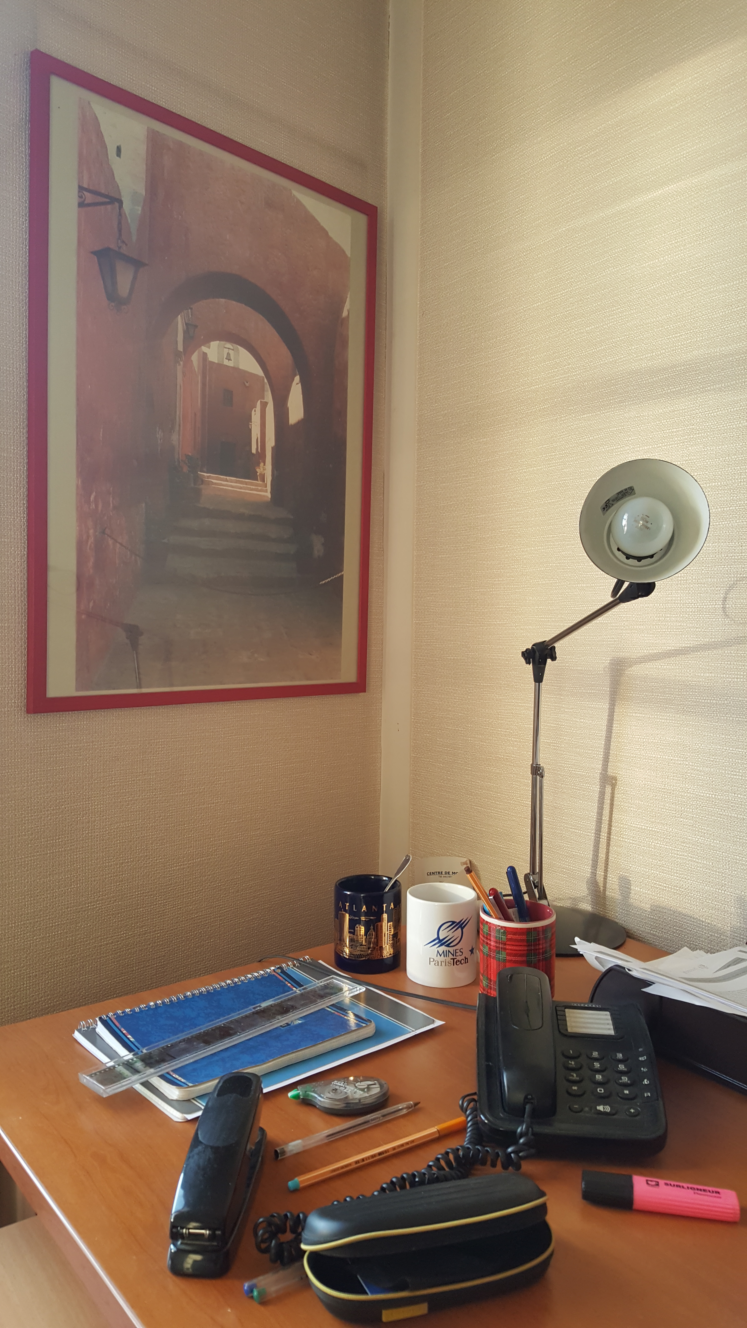
\includegraphics[height=8cm]{bureau-1}
      \end{figure}

    \end{column}
    \begin{column}{.5\textwidth}
      \begin{itemize}
      \item Where is the phone? (localization task)
      \item How many mugs are there? (quantification task)
      \item Is there a window in the room?
      \item At what time of the day was the photograph taken?
      \end{itemize}
      \pause
      \begin{alertblock}{}
        Designing computer vision systems that are able to extract semantic information from an image is a difficult task.
      \end{alertblock}

    \end{column}

  \end{columns}

\end{frame}

%%%%%%%%%%%%%%%%%%%%%%%%%%%%%%%%%%%%
\begin{frame}{Image analysis applications}

  \begin{figure}[ht]
    \centering
    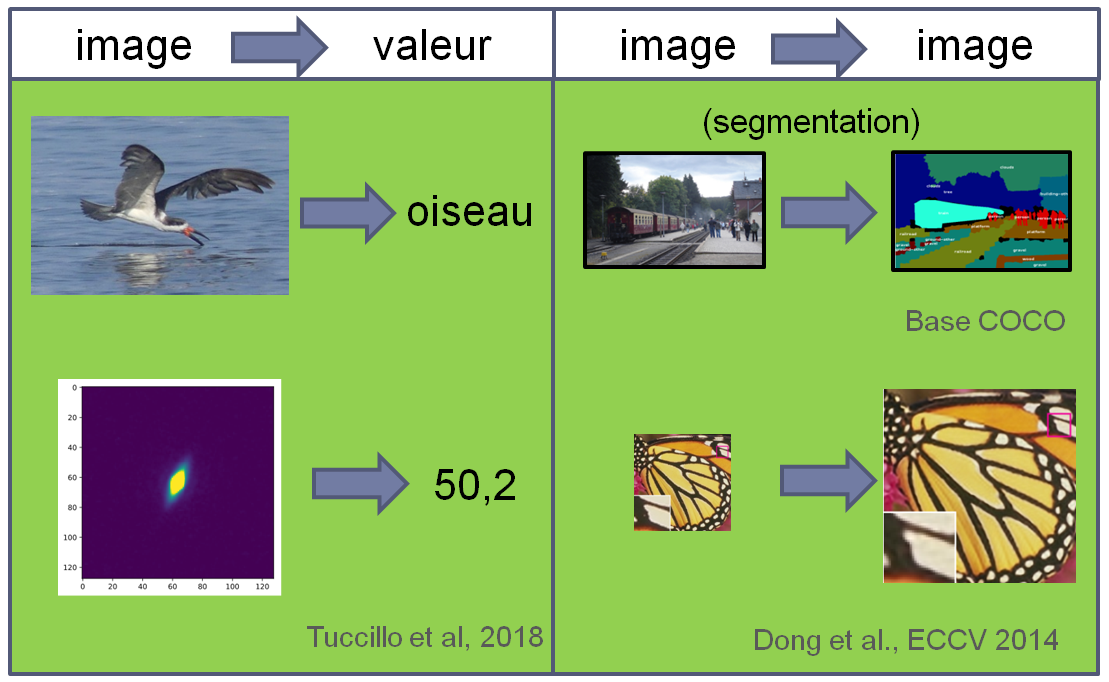
\includegraphics[width=0.76\textwidth]{applis_dl_sup}
    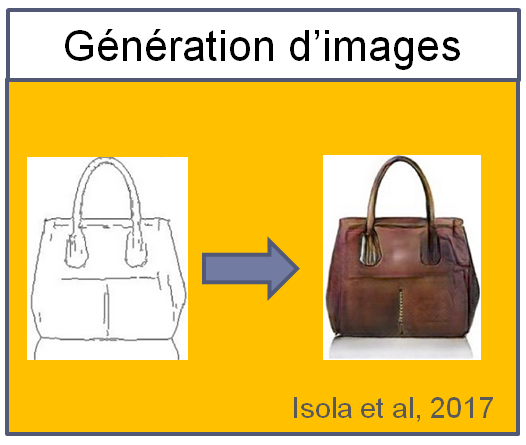
\includegraphics[width=0.33\textwidth]{applis_dl_nonsup}
  \end{figure}


\end{frame}


%%%%%%%%%%%%%%%%%%%%%%%%%%%%%%%%%%%%
\begin{frame}{Image analysis applications}

  \begin{itemize}
  \item classification
  \item quantification
  \item object localization
  \item transformation (filtering, in-painting, editing, colorization…)
  \item segmentation
  \item image caption generation
  \item 2D to 3D (stereo matching, 3D reconstruction, …)
  \item motion estimation
  \item style transfer
  \item compression
  \item anomalous image detection
  \item image generation
  \item etc.
  \end{itemize}

\end{frame}

%%%%%%%%%%%%%%%%%%%%%%%%%%%%%%%%%%%%
\begin{frame}{Classical image processing approach}

  \begin{columns}
    \begin{column}{.5\textwidth}
      Detection or segmentation task.
      \begin{block}{}
        \begin{itemize}
        \item Build a geometrical model for the objects of interest
        \item Implement this model using image processing operators
        \end{itemize}
      \end{block}

    \end{column}
    \begin{column}{.5\textwidth}
      \centering
      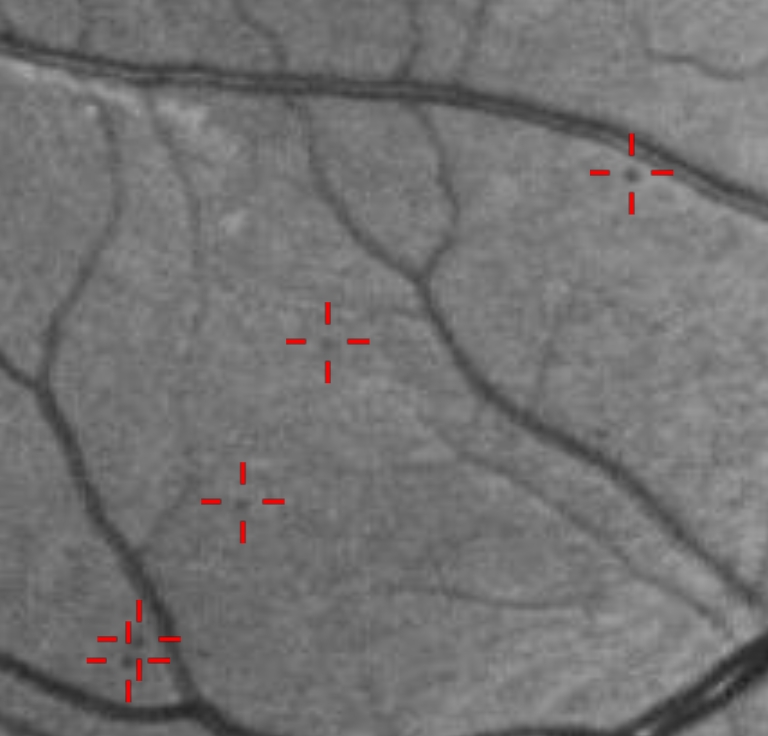
\includegraphics[width=\textwidth]{zhang_MA}\\
      \scriptsize{Detail of eye fundus image with microaneurysms to be detected}
      \source{\cite{zhang_application_2011}}

    \end{column}
  \end{columns}

  \pause

  \begin{itemize}
  \item[\boldmath$\oplus$] This approach works when the objects are not too complex
  \item[\boldmath$\oplus$] Interpretability
  \item[\boldmath$\ominus$] Often objects are difficult to model explicitly
  \end{itemize}


\end{frame}



%%%%%%%%%%%%%%%%%%%%%%%%%%%%%%%%%%%%
\frame{
  \frametitle{Classical machine learning approach}

  \begin{columns}
    \begin{column}{.35\textwidth}
      \begin{block}{}
        \begin{itemize}
        \item Compute features from the image
        \item Apply machine learning to those features
        \end{itemize}
      \end{block}

    \end{column}

    \begin{column}{.65\textwidth}
      \centering
      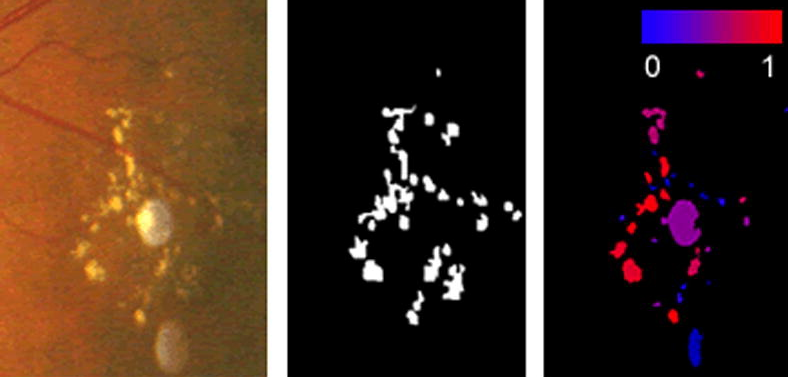
\includegraphics[width=\textwidth]{zhang_EX}\\
      \scriptsize{Exudates segmentation: original image, ground-truth and candidates with associated probabilities obtained with machine learning }
      \source{\cite{zhang_exudate_2014}}
    \end{column}
  \end{columns}
  \vspace{1em}
  \pause
  \begin{itemize}
  \item[\boldmath$\oplus$] Works well with the right features
  \item[\boldmath$\oplus$] Interpretability
  \item[\boldmath$\ominus$] An expert is required to define those features
  \item[\boldmath$\ominus$] Annotated data is required
  \end{itemize}


}

%%%%%%%%%%%%%%%%%%%%%%%%%%%%%%%%%%%%
\begin{frame}{Deep learning approach}

  \begin{block}{}
    \begin{itemize}
    \item Directly take as input the image pixels
    \item The network is supposed to build its own features
    \end{itemize}
  \end{block}

  \begin{itemize}
  \item[\boldmath$\oplus$] Good (impressive!) results
  \item[\boldmath$\ominus$] A large amount of annotated data is required
  \item[\boldmath$\ominus$] Extensive computing resources needed (for training)
  \item[\boldmath$\ominus$] Lack of interpretability
  \end{itemize}

\end{frame}

%%%%%%%%%%%%%%%%%%%%%%%%%%%%%%%%%%%%
\begin{frame}{The role of annotated image databases}

  Image databases including \emph{annotations} (typically some kind of high level information) are essential to the development of \emph{supervised} machine learning methods for image analysis.

  \begin{block}{Annotations: examples}
    \begin{itemize}
    \item Image class
    \item Measure(s) obtained from the image
    \item Position of objects within the image
    \item Segmentation
    \end{itemize}
  \end{block}

\end{frame}

%%%%%%%%%%%%%%%%%%%%%%%%%%%%%%%%%%%%
\begin{frame}{MNIST database \tiny{\cite{lecun_gradient-based_1998}}}

  \begin{itemize}
  \item The Modified National Institute of Standards and Technology (MNIST) database contains $60\,000$ training images of hand-written digits, and $10,000$ test images.
  \item Image size: $28 \times 28$
  \item It has been used since 1998
  \item Human performance on a similar database (NIST) is reported to be around $1.5\%$ error \cite{simard_efficient_1993}
  \item Best methods, based on convolutional neural networks, give around $0.21\%$ test error.
  \end{itemize}

\end{frame}

%%%%%%%%%%%%%%%%%%%%%%%%%%%%%%%%%%%%
\begin{frame}{MNIST database}

  \centering
  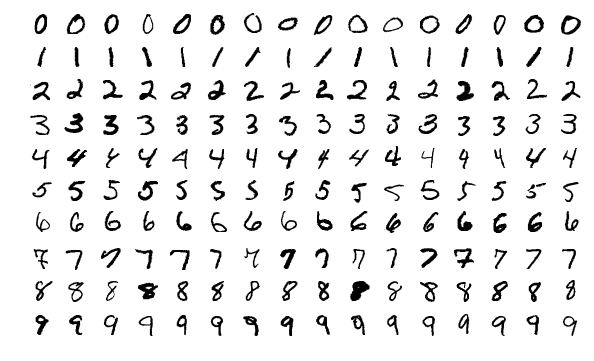
\includegraphics[width=\textwidth]{mnist_examples.png}\\
  \source{Images from MNIST assembled by Josef Stepan (licensed under CC BY-SA 4.0)}


\end{frame}

%%%%%%%%%%%%%%%%%%%%%%%%%%%%%%%%%%%%
\begin{frame}{Pascal VOC project \tiny{\cite{everingham_pascal_2010, everingham_pascal_2014}}}

  This project organized a challenge from 2005 to 2012, divided into several tasks, including an image classification task.

  \begin{block}{Pascal VOC image classification task (2012)}
    Train/val: $11\,540$ images where the presence of 20 categories of objects was annotated. The test dataset is unknown and tests are run online (still available).
  \end{block}

  \centering
  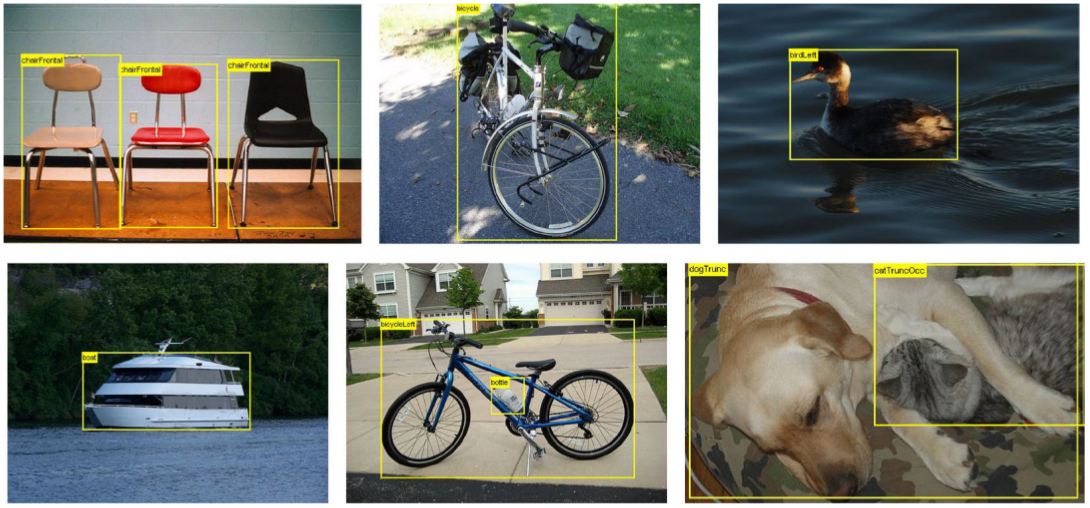
\includegraphics[width=0.75\textwidth]{pascal_examples.png}
  \source{From \cite{everingham_pascal_2014}}

\end{frame}

%%%%%%%%%%%%%%%%%%%%%%%%%%%%%%%%%%%%
\begin{frame}{ImageNet project \tiny{\cite{russakovsky_imagenet_2015}}}

  Between 2010 and 2017 ImageNet organized an annual challenge: The ImageNet Large Scale Visual Recognition Challenge (ILSVRC). It represented a breakthrough in the design of image analysis challenges by its size.

  \begin{block}{Image classification task}
    \begin{itemize}
    \item
      Training: $1\,281\,167$; validation: $50\,000$; test: $100\,000$.
    \item
      $1\,000$ classes (90 dog breeds!).
    \end{itemize}
  \end{block}

\end{frame}

%%%%%%%%%%%%%%%%%%%%%%%%%%%%%%%%%%%%
\begin{frame}{ImageNet projet}

  \centering
  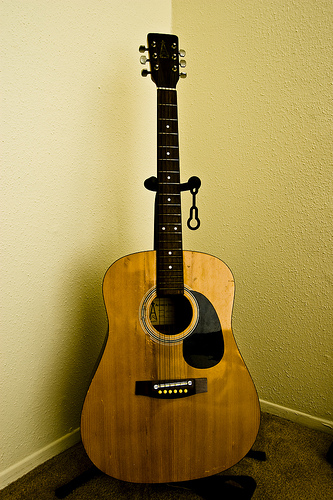
\includegraphics[width=0.20\textwidth]{ilsvrc_guitar2}\hspace{0.1em}
  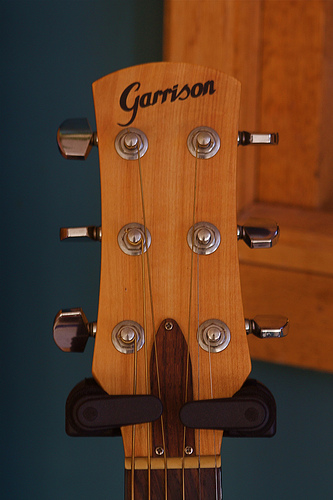
\includegraphics[width=0.20\textwidth]{ilsvrc_guitar3}\\
  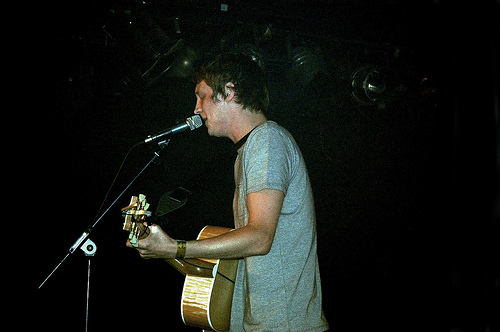
\includegraphics[width=0.39\textwidth]{ilsvrc_guitar1}\hspace{0.1em}
  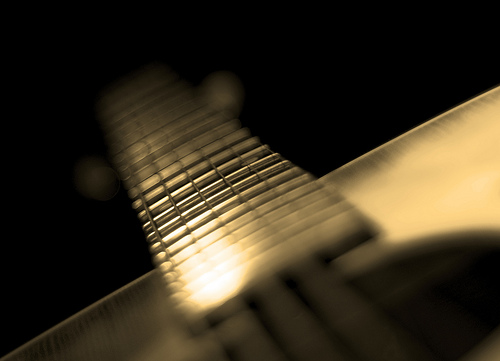
\includegraphics[width=0.39\textwidth]{ilsvrc_guitar4}\\
  Examples from the \emph{acoustic guitar} class


\end{frame}

%%%%%%%%%%%%%%%%%%%%%%%%%%%%%%%%%%%%%%%%%%%%%%%%%%
\frame{
  \frametitle{Deep learning achievements}

  \begin{columns}
    \begin{column}{.5\textwidth}
      \begin{block}{ImageNet Large Scale Visual Recognition Challenge (ILSVRC)}
        2012: \emph{AlexNet} \cite{krizhevsky_imagenet_2012} won this challenge by a large margin
      \end{block}

    \end{column}

    \begin{column}{.5\textwidth}
      \centering
      \scriptsize
      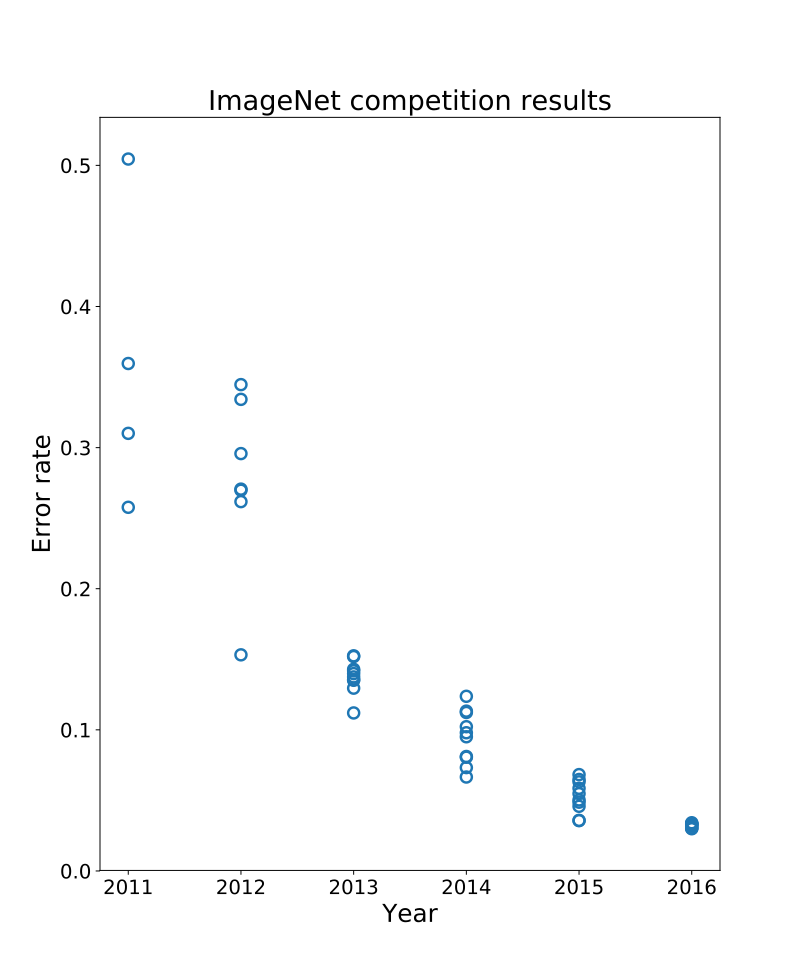
\includegraphics[height=0.75\textheight]{ImageNet_error_history}
      Evolution of top-5 error rate

      \source{Wikipedia (CC BY-SA 4.0)}

    \end{column}
  \end{columns}

}
%%%%%%%%%%%%%%%%%%%%%%%%%%%%%%%%%%%%%%%%%%%%%%%%%%

\frame{
  \frametitle{Deep learning achievements (cont.)}

  \begin{itemize}
  \item 2011: first super-human performance, IJCNN 2011 traffic sign recognition contest \cite{ciresan_committee_2011}
    \begin{figure}[ht]
      \centering
      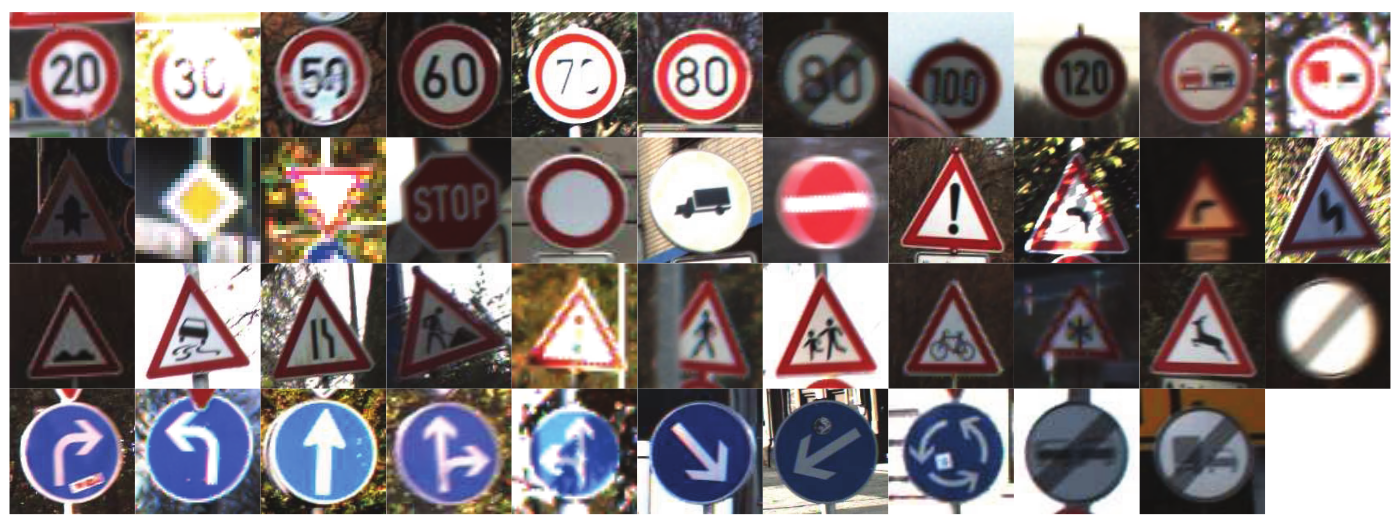
\includegraphics[width=0.7\textwidth]{ijcnn2011.png}
      \source{\cite{stallkamp_german_2011}}
    \end{figure}

  %% \item 2012: visual object detection (Mitosis detection in breast cancer histology \cite{ciresan_mitosis_2013})
  \item 2012: segmentation competition (neuronal membranes in electron microscopy images \cite{ciresan_deep_2012})
  \end{itemize}

}

%%%%%%%%%%%%%%%%%%%%%%%%%%%%%%%%%%%%%%%%%%%%%%%%%%

\begin{frame}{Deep learning achievements (cont.)}

  \begin{columns}
    \begin{column}{.4\textwidth}
      \begin{itemize}
      \item 2016: AlphaGo beats Lee Sedol, one of the best go players, in a 5-game match
      \end{itemize}
    \end{column}

    \begin{column}{.6\textwidth}

      \begin{figure}[ht]
        \centering
        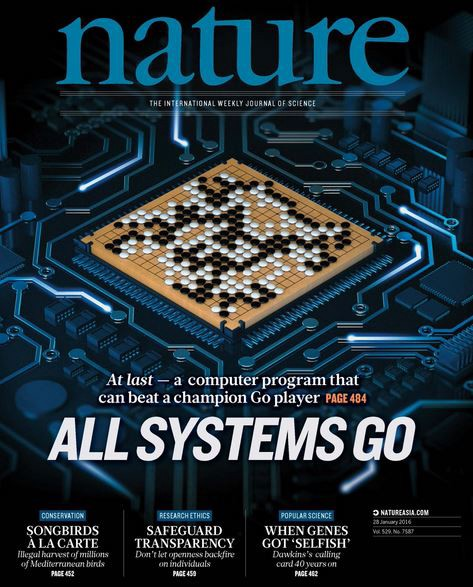
\includegraphics[width=\textwidth]{nature_go.jpg}
      \end{figure}
    \end{column}
  \end{columns}

\end{frame}


%%%%%%%%%%%%%%%%%%%%%%%%%%%%%%%%%%%%%%%%%%%%%%%%
\section{Application of fully connected NNs to image classification}


%%%%%%%%%%%%%%%%%%%%%%%%%%%%%%%%%%%%%%%%%%%%%%%%%%

\frame{
  \frametitle{Reminder: Artificial neuron}

  \begin{figure}
    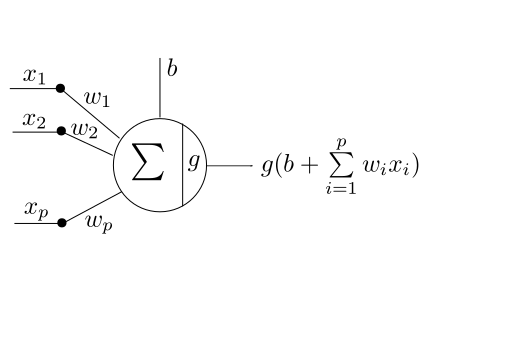
\includegraphics[height=3cm]{neurone_representation_compacte}
  \end{figure}

  \begin{itemize}

  \item $b, w_1, \ldots, w_n$ are the neuron parameters, to be learnt

  \item $\act$ is the activation function

  \end{itemize}


}


%%%%%%%%%%%%%%%%%%%%%%%%%%%%%%%%%%%%
\begin{frame}{Image classification problem}

  Classification problem:
  \begin{itemize}
  \item Input: image
  \item Output: class $y$ chosen from a set of labels: $\{ label_1, label_2, \ldots, label_q\}$
  \end{itemize}

  %% \begin{block}{Class coding}
  %%   Often, classes are denoted by integers, but this is only a coding commodity. For instance, it would be meaningless to use a regression approach for this problem.
  %% \end{block}

\end{frame}

%%%%%%%%%%%%%%%%%%%%%%%%%%%%%%%%%%%%%%%%%%%%%%%%%%

\frame<beamer>{
  \frametitle{Input image, input neurons}

  In the scalar case (single-valued images), each input pixel is considered as an input neuron.

  \vspace{10pt}

  \begin{columns}

    \begin{column}<1->{0.45\textwidth}
      \begin{center}
        \includegraphics<1-2>[width=0.9\textwidth]{cnn_pixels.png}
        \includegraphics<3->[width=0.9\textwidth]{imagette.png}
      \end{center}
    \end{column}

    \begin{column}<2->{0.45\textwidth}
      \begin{center}
        \includegraphics<2>[width=0.9\textwidth]{cnn_neurones.png}
        \includegraphics<3->[width=0.9\textwidth]{imagette_neurones.png}

      \end{center}
    \end{column}

  \end{columns}

  %% \pause

  %% \begin{alertblock}<4->{Image preprocessing}
  %%   Often, the input image is modified to make the optimization of the model easier.
  %% \end{alertblock}

}


%%%%%%%%%%%%%%%%%%%%%%%%%%%%%%%%%%%%%%%%%%%%%%%%%%

\frame<handout>{
  \frametitle{Input image, input neurons}

  In the scalar case (single-valued images), each input pixel is considered as an input neuron.

  \vspace{10pt}

  \begin{columns}

    \begin{column}{0.45\textwidth}
      \begin{center}
        
\includegraphics[width=0.9\textwidth]{imagette.png}
      \end{center}
    \end{column}

    \begin{column}{0.45\textwidth}
      \begin{center}
        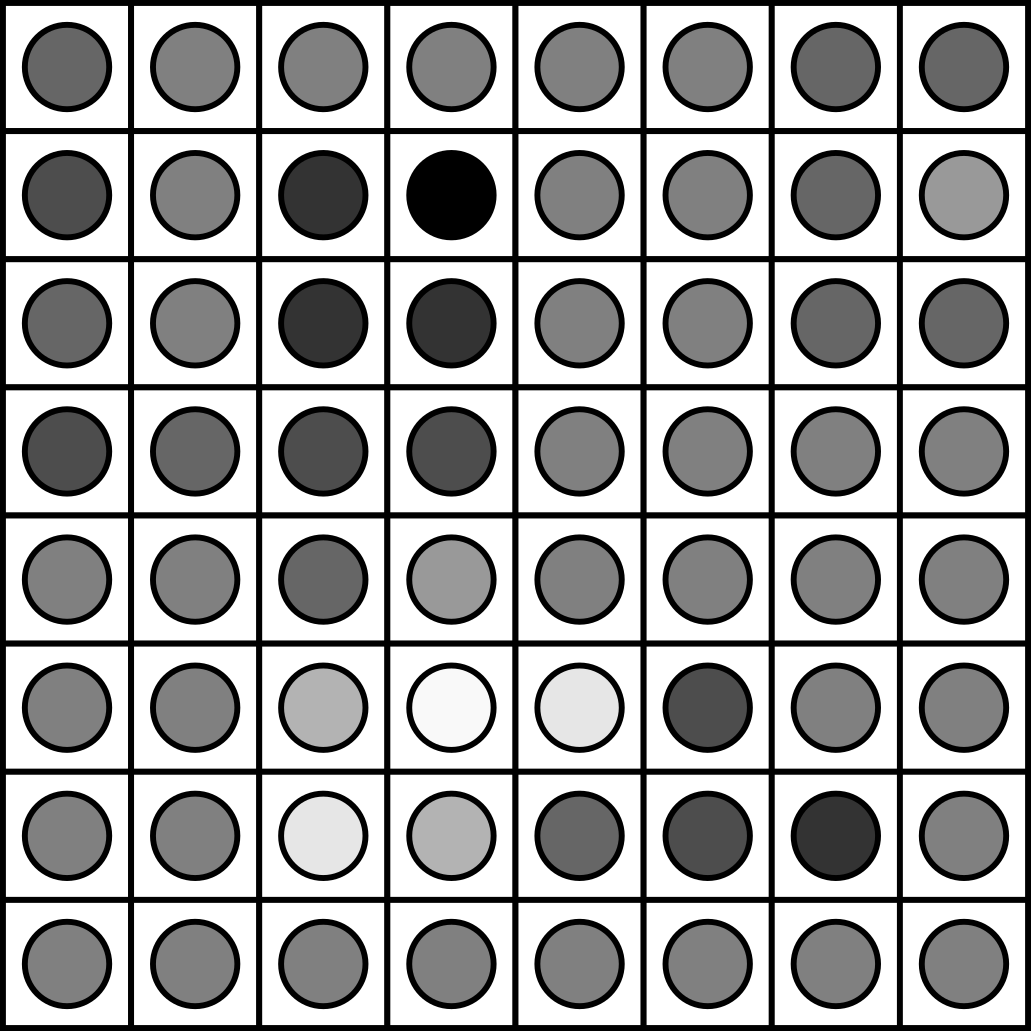
\includegraphics[width=0.9\textwidth]{imagette_neurones.png}

      \end{center}
    \end{column}

  \end{columns}

  %% \pause

  %% \begin{alertblock}<4->{Image preprocessing}
  %%   Often, the input image is modified to make the optimization of the model easier.
  %% \end{alertblock}

}

%%%%%%%%%%%%%%%%%%%%%%%%%%%%%%%%%%%%%%%%%%%%%%%%%%

\frame{
  \frametitle{How are we going to apply our NN to an image?}

\begin{columns}
  \begin{column}{.5\textwidth}
      \begin{center}
        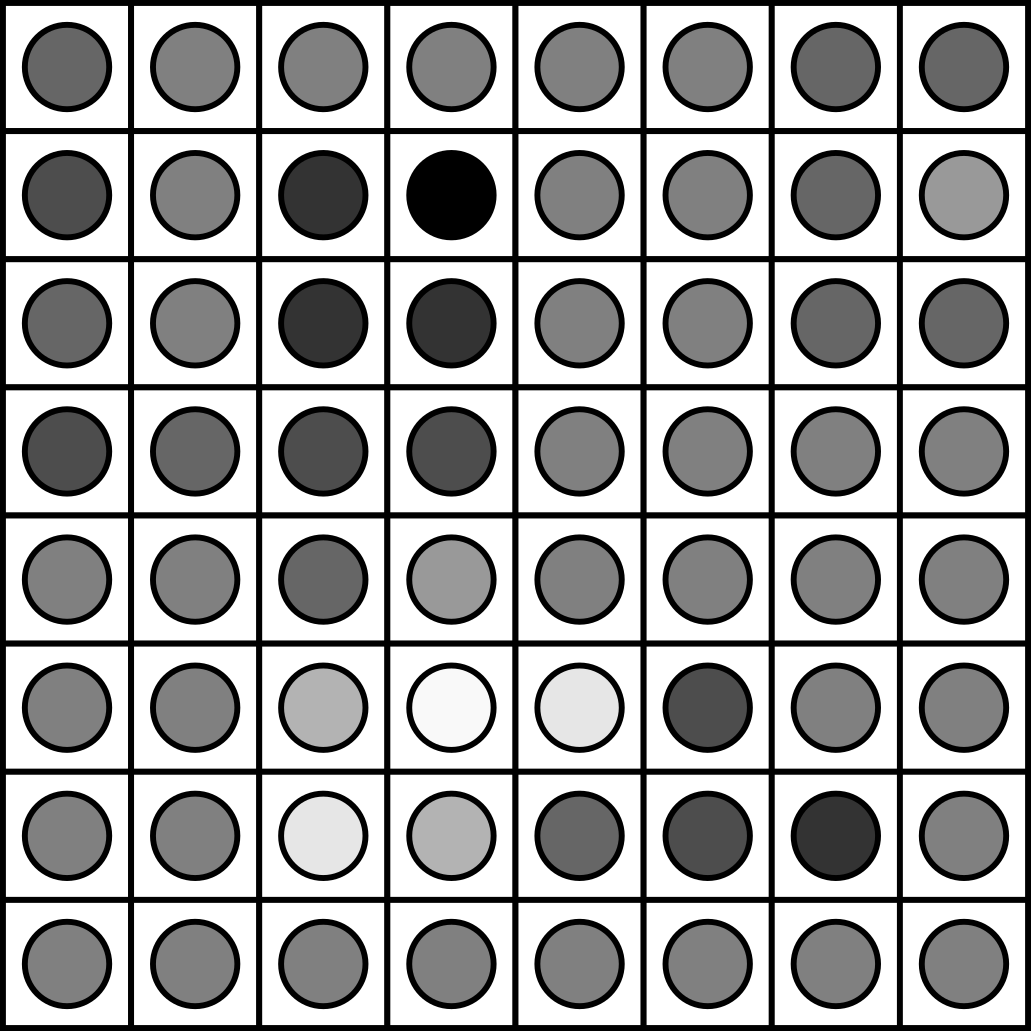
\includegraphics[width=0.9\textwidth]{imagette_neurones.png}

      \end{center}

  \end{column}

  \begin{column}{.5\textwidth}
  \begin{figure}
    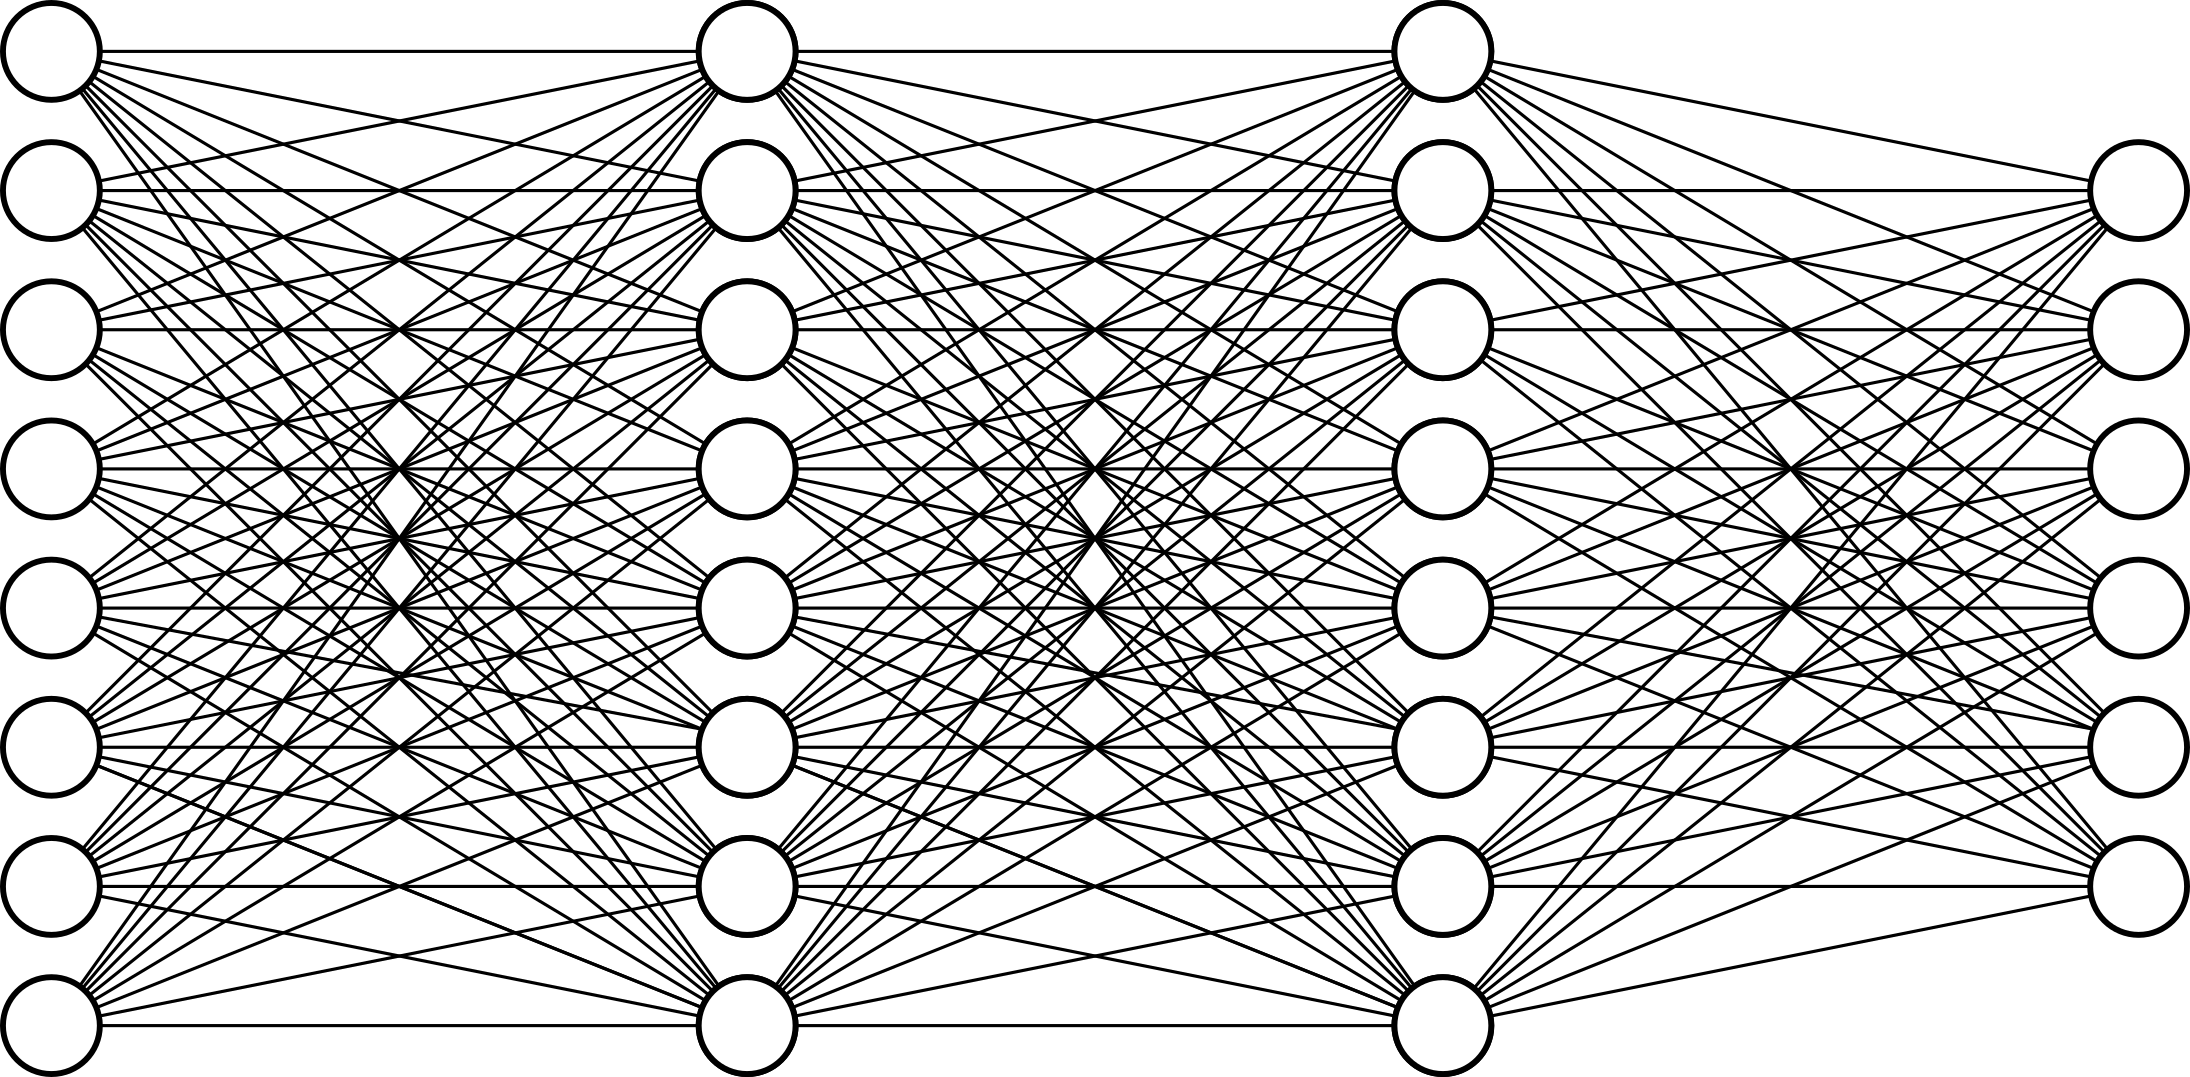
\includegraphics[width=\textwidth]{mini_reseau3_bis}
  \end{figure}

  \end{column}
\end{columns}


}


%%%%%%%%%%%%%%%%%%%%%%%%%%%%%%%%%%%%%%%%%%%%%%%%%%

\frame{
  \frametitle{}

  \vspace{10pt}

  \begin{columns}

    \begin{column}{0.45\textwidth}
      \begin{center}
        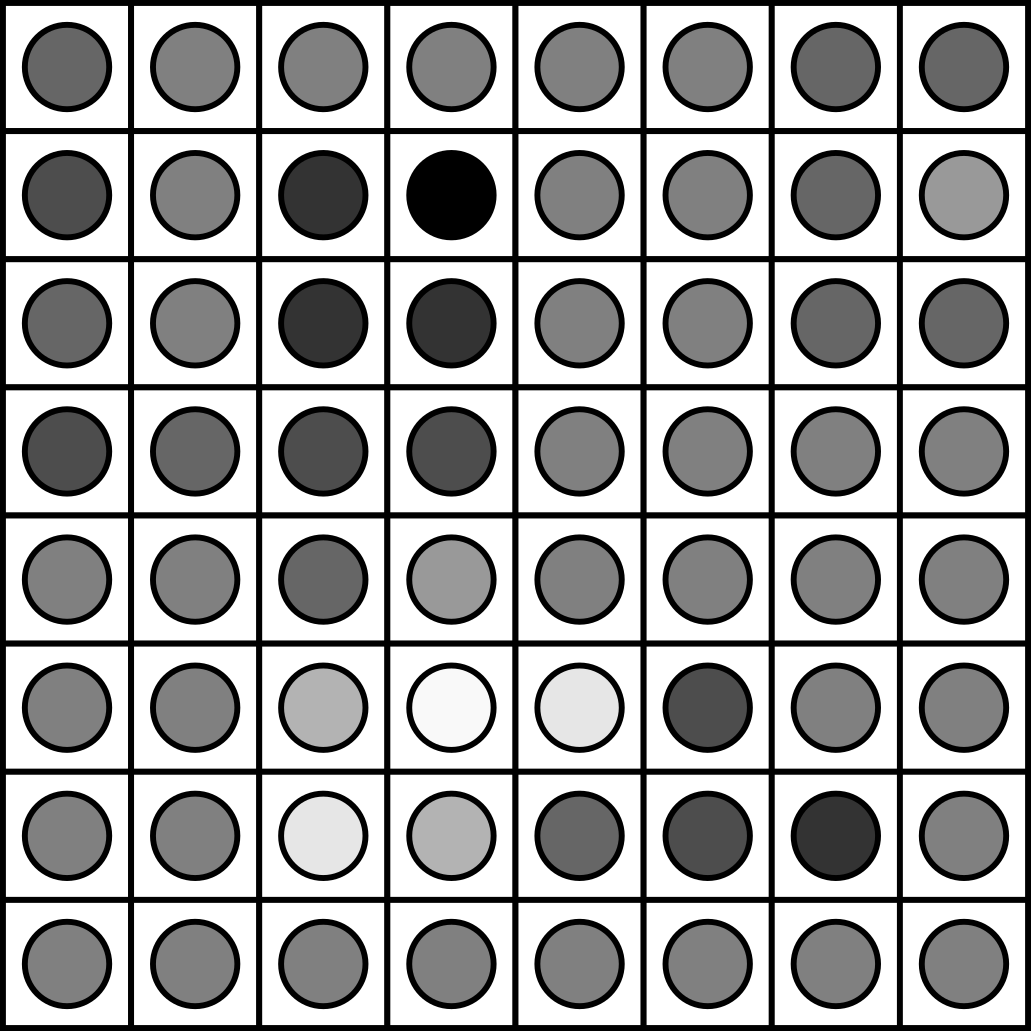
\includegraphics[width=0.9\textwidth]{imagette_neurones.png}
      \end{center}
    \end{column}

    \begin{column}{0.55\textwidth}

      \begin{quizzblock}{What approach would you suggest to apply our fully connected NN to an image?}
    \begin{itemize}
    \item[1/] Integrate along the horizontal or vertical axis, in order to get rid of a dimension
    \item[2/] Apply the network to each row or column separately
    \item[3/] Transform the image into a vector, by rearranging the pixels
    \end{itemize}

  \end{quizzblock}

    \end{column}

  \end{columns}

  %% \pause

  %% \begin{alertblock}<4->{Image preprocessing}
  %%   Often, the input image is modified to make the optimization of the model easier.
  %% \end{alertblock}

}


%%%%%%%%%%%%%%%%%%%%%%%%%%%%%%%%%%%%
\begin{frame}{Class coding}

  If there are $q$ possible classes, then a class will be coded as a vector $\y$ of length $q$. If its class is $r$  then for $0 \leq i < q$:
  \[
  \y[i] =
  \begin{cases}
    1, & \text{if}\ i=r \\
    0, & \text{otherwise}
  \end{cases}
  \]

  \begin{block}{Example with $3$ classes}
    \begin{itemize}
    \item
      Label $0 \longmapsto [1,0,0]$
    \item
      Label $1 \longmapsto [0,1,0]$
    \item
      Label $2 \longmapsto [0,0,1]$
    \end{itemize}
  \end{block}

  This is called \alert{one-hot encoding}. The resulting vector is a one-hot vector.

\end{frame}


%%%%%%%%%%%%%%%%%%%%%%%%%%%%%%%%%%%%
\begin{frame}{}

\begin{quizzblock}{Why is one-hot encoding used, instead of integers?}
  \begin{itemize}
  \item[1/ ] The network performs better in the $[0,1]$ range
  \item[2/ ] One-hot encoding makes the labels symmetric, i.e. permutation invariant.
  \end{itemize}
\end{quizzblock}

  \vspace{1em}

  \begin{columns}
    \begin{column}{.5\textwidth}
  \begin{block}{One-hot encoding}
    \begin{itemize}
    \item
      Label $0 \longmapsto [1,0,0]$
    \item
      Label $1 \longmapsto [0,1,0]$
    \item
      Label $2 \longmapsto [0,0,1]$
    \end{itemize}
  \end{block}

    \end{column}

    \begin{column}{.5\textwidth}
  \begin{block}{Integer encoding}
    \begin{itemize}
    \item
      Label $0 \longmapsto 0$
    \item
      Label $1 \longmapsto 1$
    \item
      Label $2 \longmapsto 2$
    \end{itemize}
  \end{block}

    \end{column}
  \end{columns}

  \pause

  \vspace{1em}

  \mode<beamer>{
    \begin{itemize}
    \item Using integers to represent the labels would bring an \alert{inductive bias} into the model: there will be an explicit order between the labels.
    \item Using one-hot encoding, we make the labels permutation invariant
  \end{itemize}}

\end{frame}


%%%%%%%%%%%%%%%%%%%%%%%%%%%%%%%%%%%%
\begin{frame}{Activations}

  Different activations (typically ReLU) can be used in the intermediate layers.
  \vspace{1em}

  Concerning the last layer: Given that the aim is a vector containing zeros except for a one, two designs are commonly used:

  \begin{itemize}
  \item Use a sigmoid as last activation
  \item Last layer: a softmax operator
  \end{itemize}

\end{frame}

%%%%%%%%%%%%%%%%%%%%%%%%%%%%%%%%%%%%
\begin{frame}{Softmax operator}

  \begin{block}{Definition}
    The softmax operator $\sigma: \R^d \rightarrow \R^d$ is given by:
    \[
    \forall \mathbf{x}  \in \R^d, \forall k \in \{1, \ldots, d\}:\quad \sigma(\mathbf{x})_k = \frac{e^{\mathbf{x}_k}}{\sum\limits_{i=1}^d e^{\mathbf{x}_i}}
    \]
  \end{block}

  \pause

  \begin{columns}
    \begin{column}{.3\textwidth}
      \begin{block}{Some properties}
        \begin{itemize}
        \item $0 < \sigma(\mathbf{x})_k < 1$
        \item $\sum\limits_{i=1}^d \sigma(\mathbf{x})_i = 1$
        \end{itemize}
      \end{block}

    \end{column}

    \pause

    \begin{column}{.7\textwidth}

      \begin{block}{Example}
        \[
        \mathbf{x} = \myvec{10.1\\0\\-4.3\\1.33}  \quad \sigma(\mathbf{x}) \approx \myvec{0.9998\\0.000041\\0.00000056\\0.00016}
        \]

      \end{block}



    \end{column}
  \end{columns}



\end{frame}

%%%%%%%%%%%%%%%%%%%%%%%%%%%%%%%%%%%%
\begin{frame}{Loss function for classification: cross-entropy}

  The preferred loss function for classification is cross-entropy:

  \begin{block}{}
    For $\y$ in $\{0, 1\}^d$ and $\hat{\y}$ in $]0, 1[^d$:
    \[
    H(\y, \hat{\y}) = - \sum_{i=1}^d \y_i \log(\hat{\y}_i)
    \]

    \small
    Reminder -- hat notation: $\hat{\y}$ is the prediction that is supposed to be close to $\y$.
  \end{block}

  \pause

  Remarks:
  \begin{itemize}
  \item   Here $\y$ is a one-hot vector: $\y_i = 1$ for $i=r$ and $\y_i=0$ otherwise. Therefore the cross-entropy will ``push'' $\hat{\y}_r$ towards $1$. Why will the other elements of $\hat{\y}$ be pushed towards $0$?  \pause \mode<beamer>{Because $\hat{\y}$ is typically computed by a softmax.}
    \pause
  \item   The binary cross-entropy we previously saw is a particular case of cross-entropy.

  \end{itemize}

\end{frame}

%%%%%%%%%%%%%%%%%%%%%%%%%%%%%%%%%%%%
\begin{frame}{Image classification with a fully-connected NN}

  \begin{block}{Input}
    The input image, containing $p$ pixels, is transformed into a vector of length $p$.
  \end{block}

  \begin{block}{Output}
    For $q$ classes, the output will be a vector of length $q$.
  \end{block}

  \pause

  \begin{block}{Example: image of size $4 \times 2$, $6$ possible classes}
    \centering
    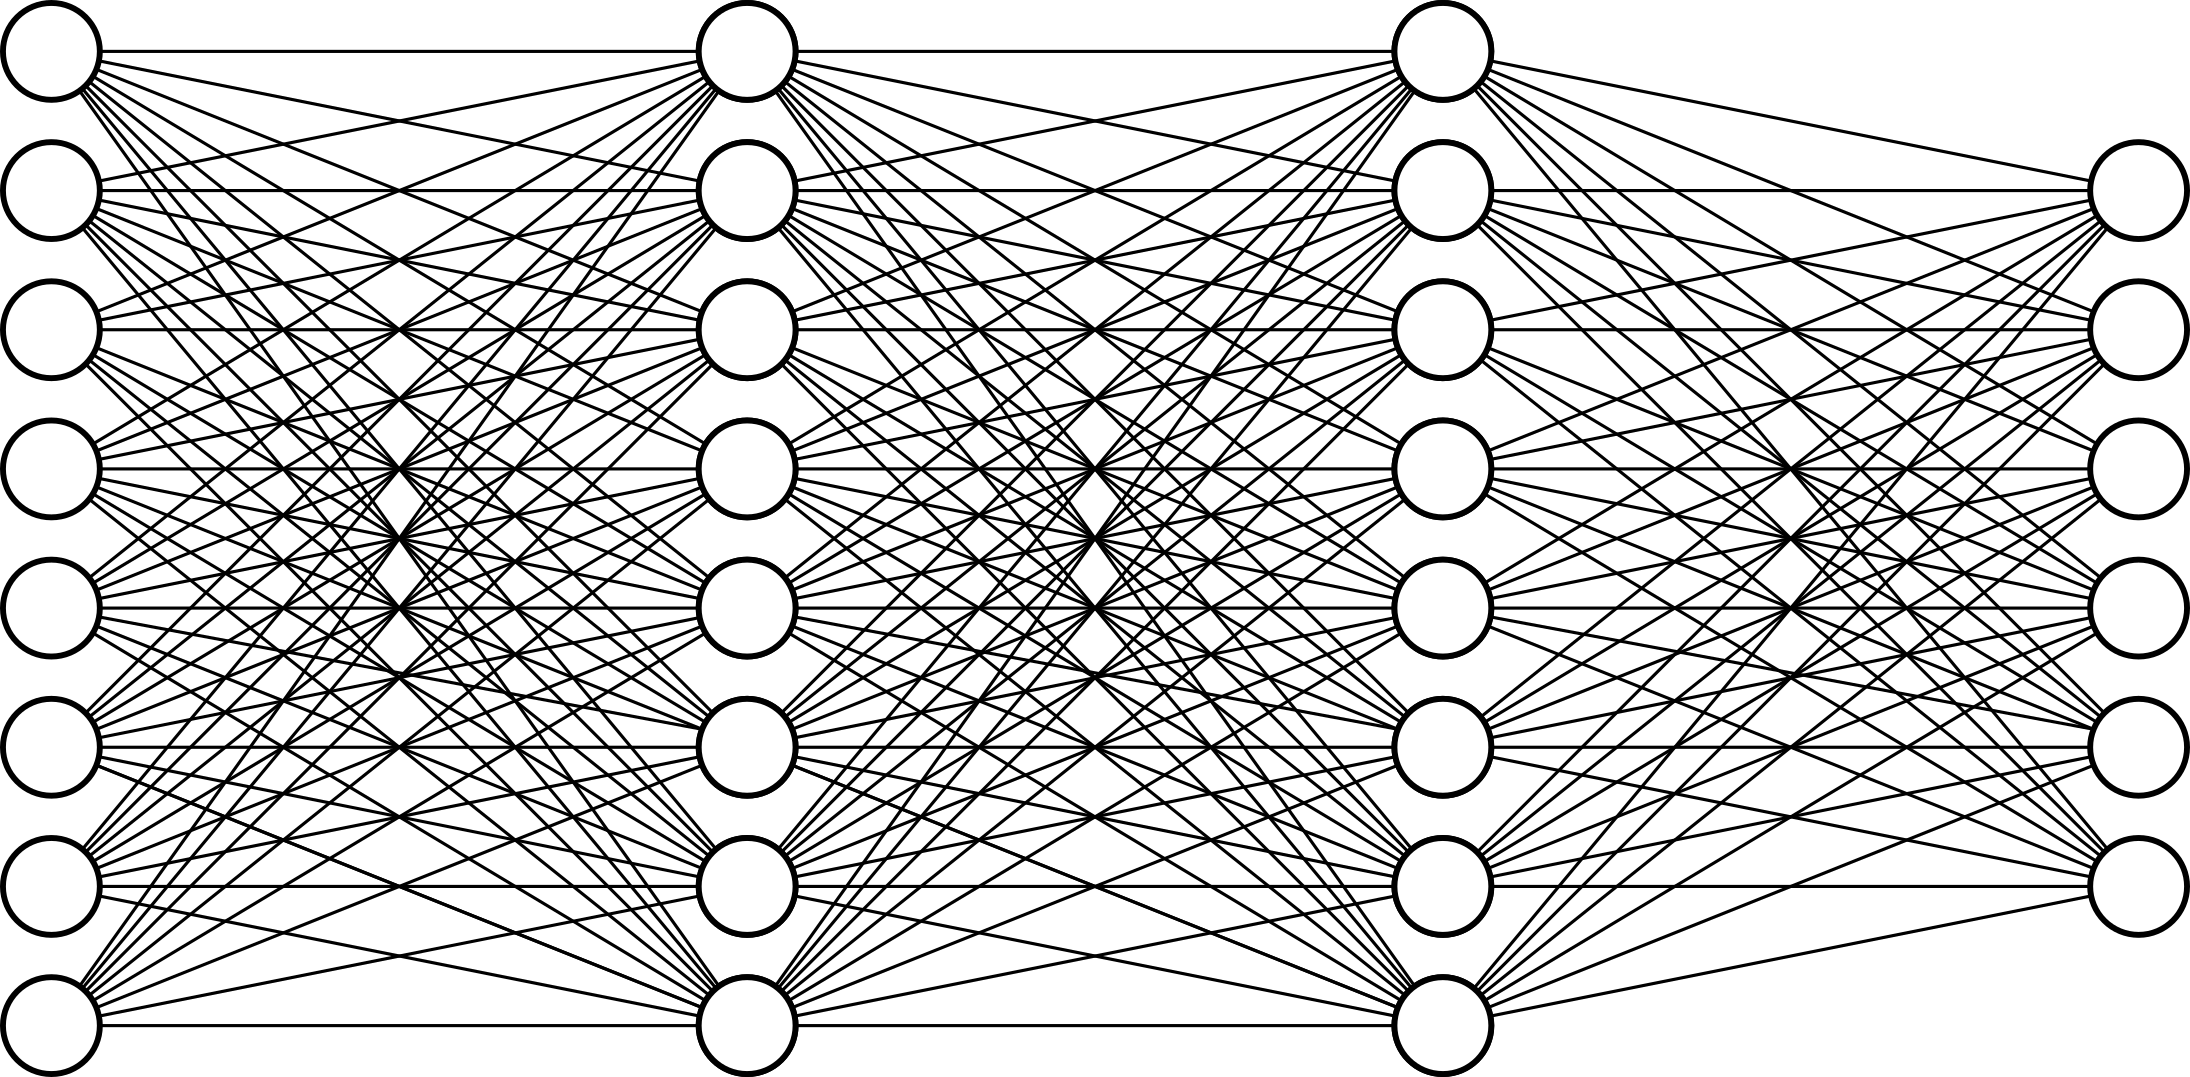
\includegraphics[width=0.6\textwidth]{mini_reseau3_bis}
  \end{block}

\end{frame}


%%%%%%%%%%%%%%%%%%%%%%%%%%%%%%%%%%%%
\begin{frame}{Image classification using a fully-connected NN}

  \centering
  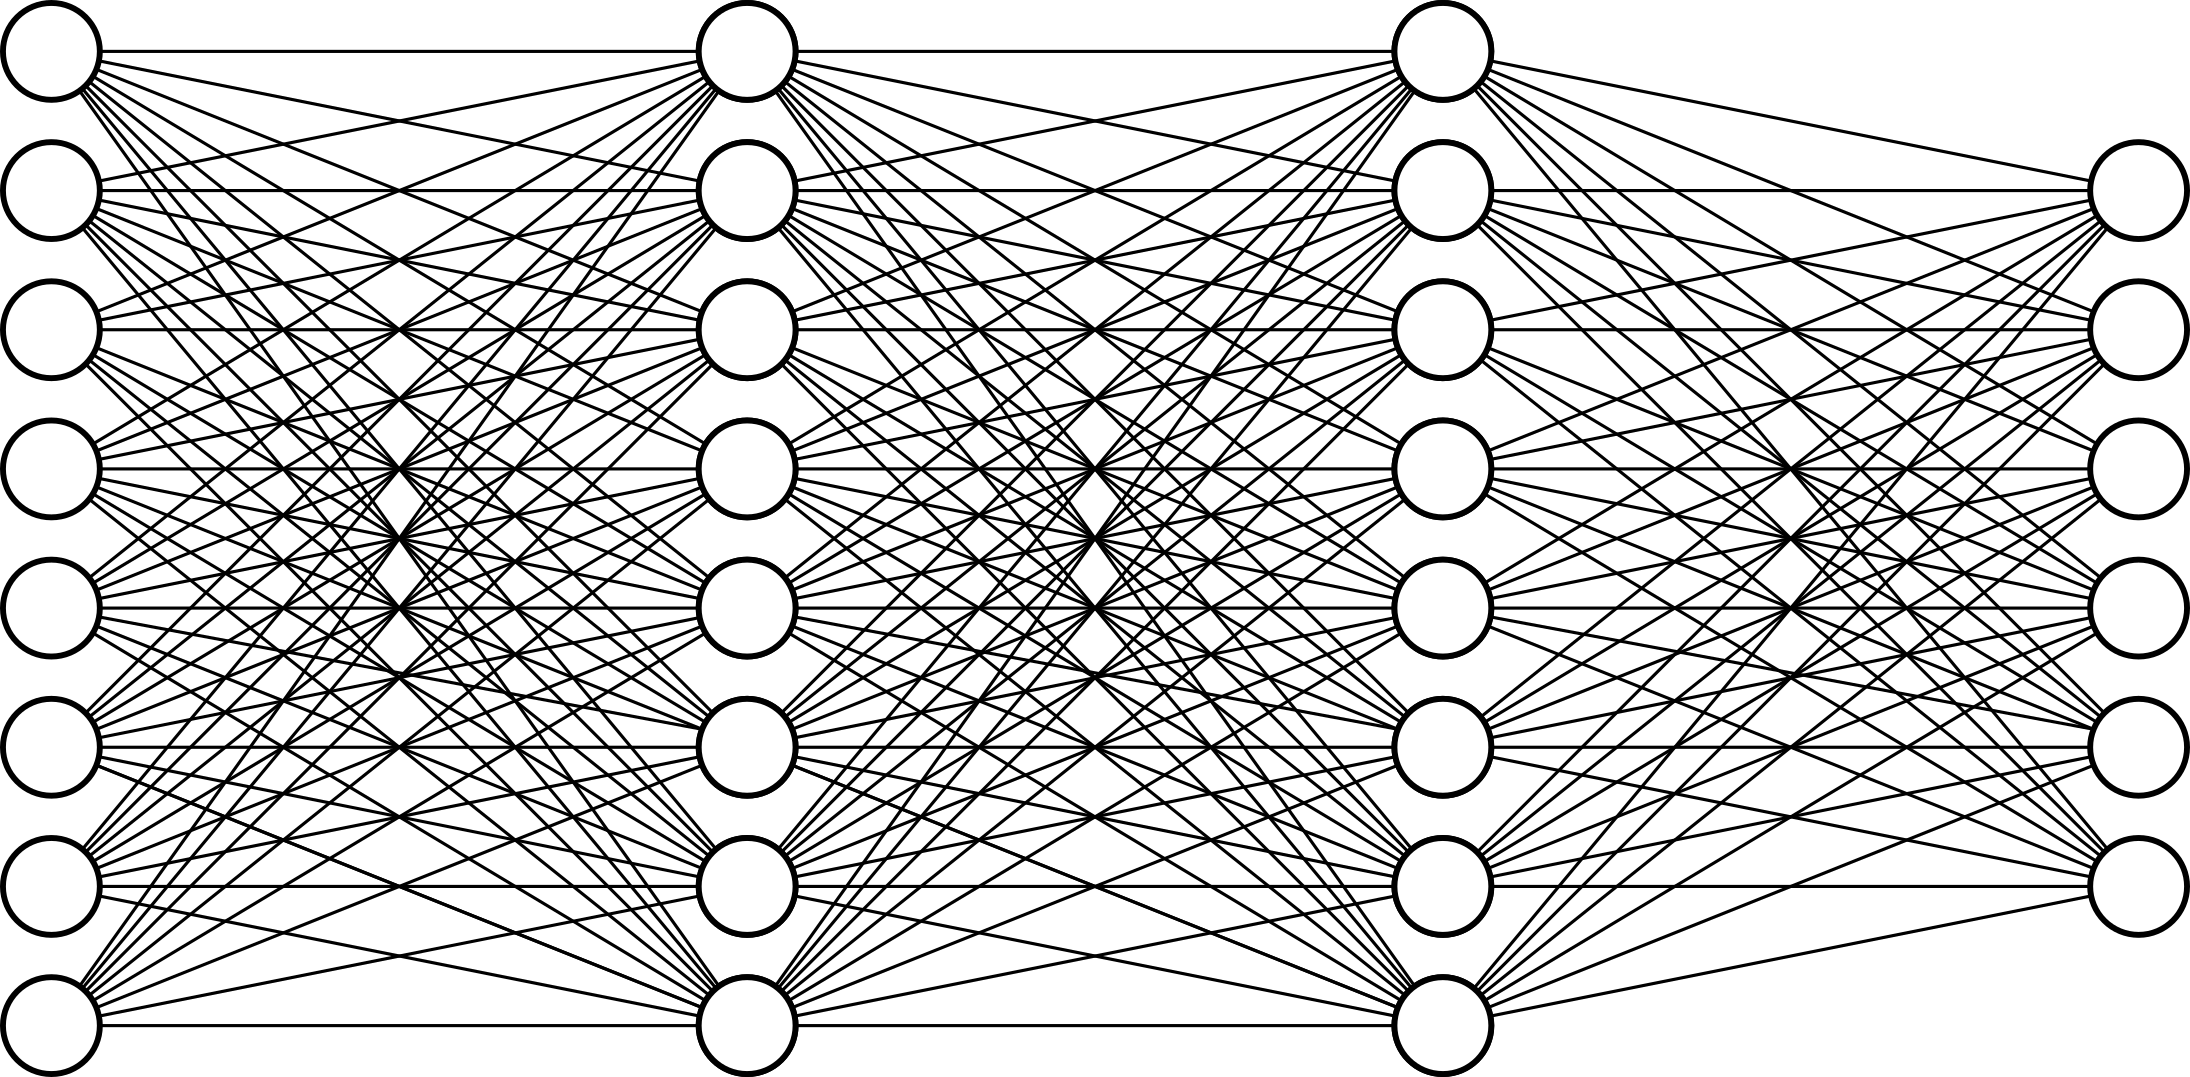
\includegraphics[width=0.6\textwidth]{mini_reseau3_bis}

  \begin{itemize}[<+->]
  \item A small image easily contains $100\,000$ pixels
  \item The number of parameters between two layers of that size is $10^5 \times (10^5 + 1)$!
  \item This approach is only possible for very small images
%  \item This approach does not take into account the local structure of images
  \end{itemize}

\end{frame}

%%%%%%%%%%%%%%%%%%%%%%%%%%%%%%%%%%%%%%%%%%%%%%%%%%
\frame{
  \frametitle{Conclusion on fully-connected networks for image classification}

  Fully-connected layers scale badly to large size images.


  Today:

  \begin{itemize}
  \item NN solely composed of fully-connected layers are almost never used for image analysis \footnote{However, \alert{transformers}~\cite{dosovitskiy_image_2021} have brought new ways to use fully-connected layers.}.
  \item Fully-connected layers are mainly used in the middle (auto-encoders) or at the end (classification) of the pipeline.
  \end{itemize}

}



%%%%%%%%%%%%%%%%%%%%%%%%%%%%%%%%%%%%%%%%%%%%%%%%%%
%%%%%%%%%%%%%%%%%%%%%%%%%%%%%%%%%%%%%%%%%%%%%%%%%%
\section{From fully-connected layers to convolutional layers}

%%%%%%%%%%%%%%%%%%%%%%%%%%%%%%%%%%%%
\begin{frame}{Layers representation}

  \begin{block}{}
    \begin{itemize}
    \item     For illustration purposes, in the following slides images and layers will be displayed as rows of neurons -- as sections of 2D arrays.
    \item     Only some connections between neurons are represented. Each such connection is associated to a weight. The biases are not represented, to avoid clutter.
    \end{itemize}

  \end{block}

  \begin{columns}

    \begin{column}<1->{0.33\textwidth}
      \begin{center}
        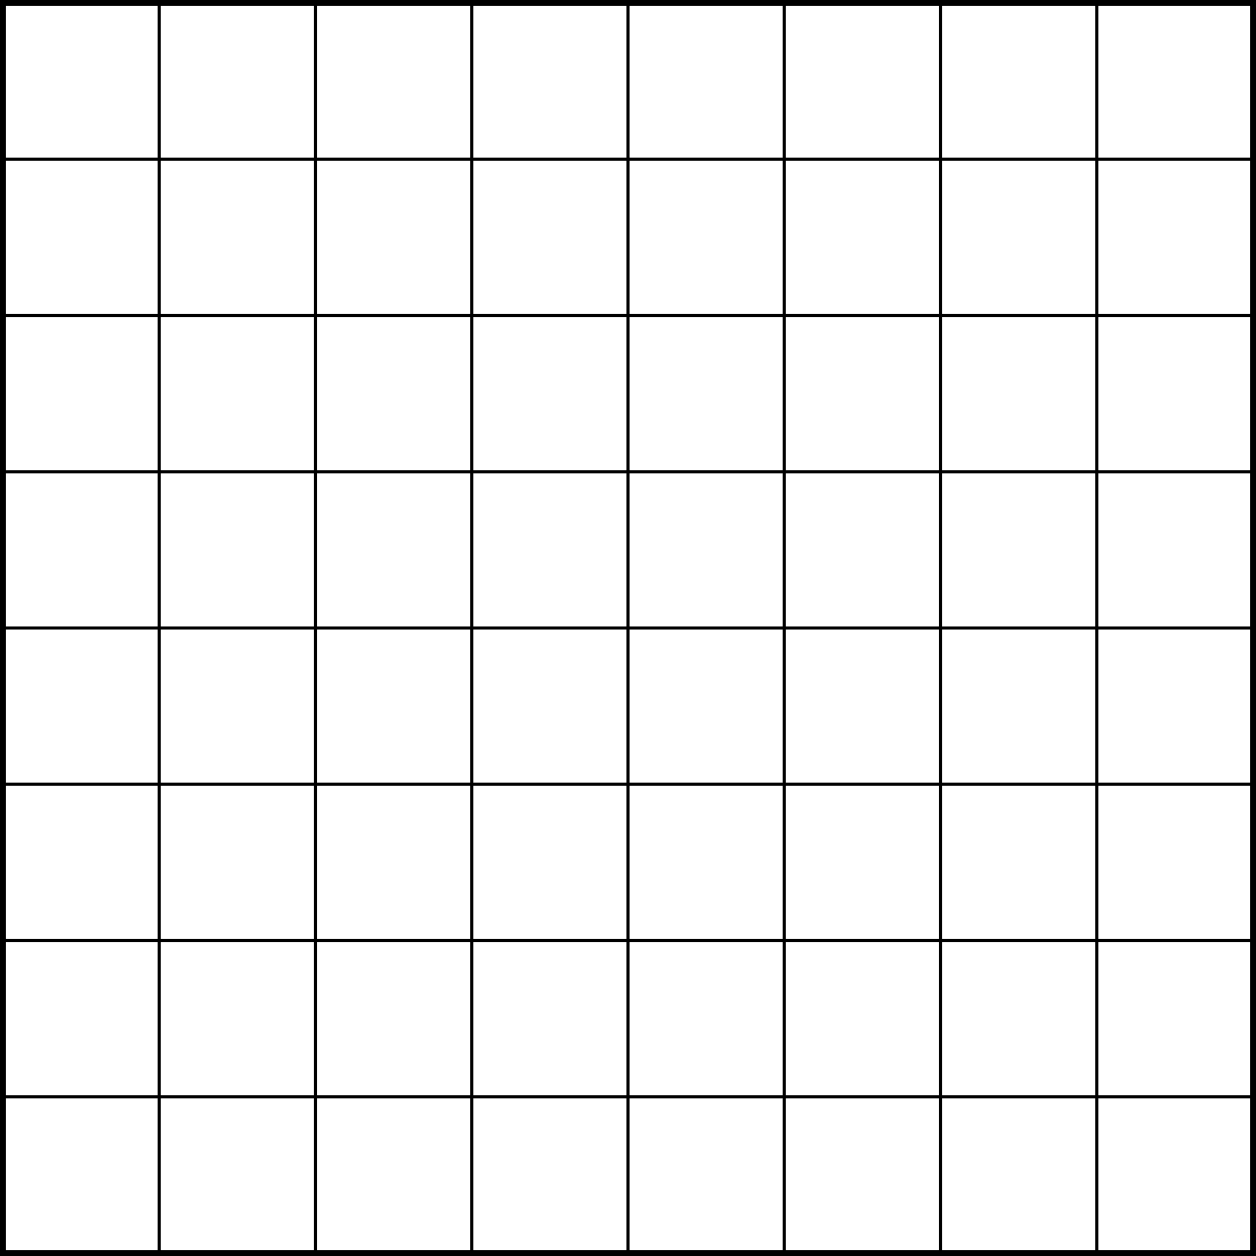
\includegraphics[width=0.80\textwidth]{cnn_pixels.png}
      \end{center}
    \end{column}

    \begin{column}<2->{0.33\textwidth}
      \begin{center}
        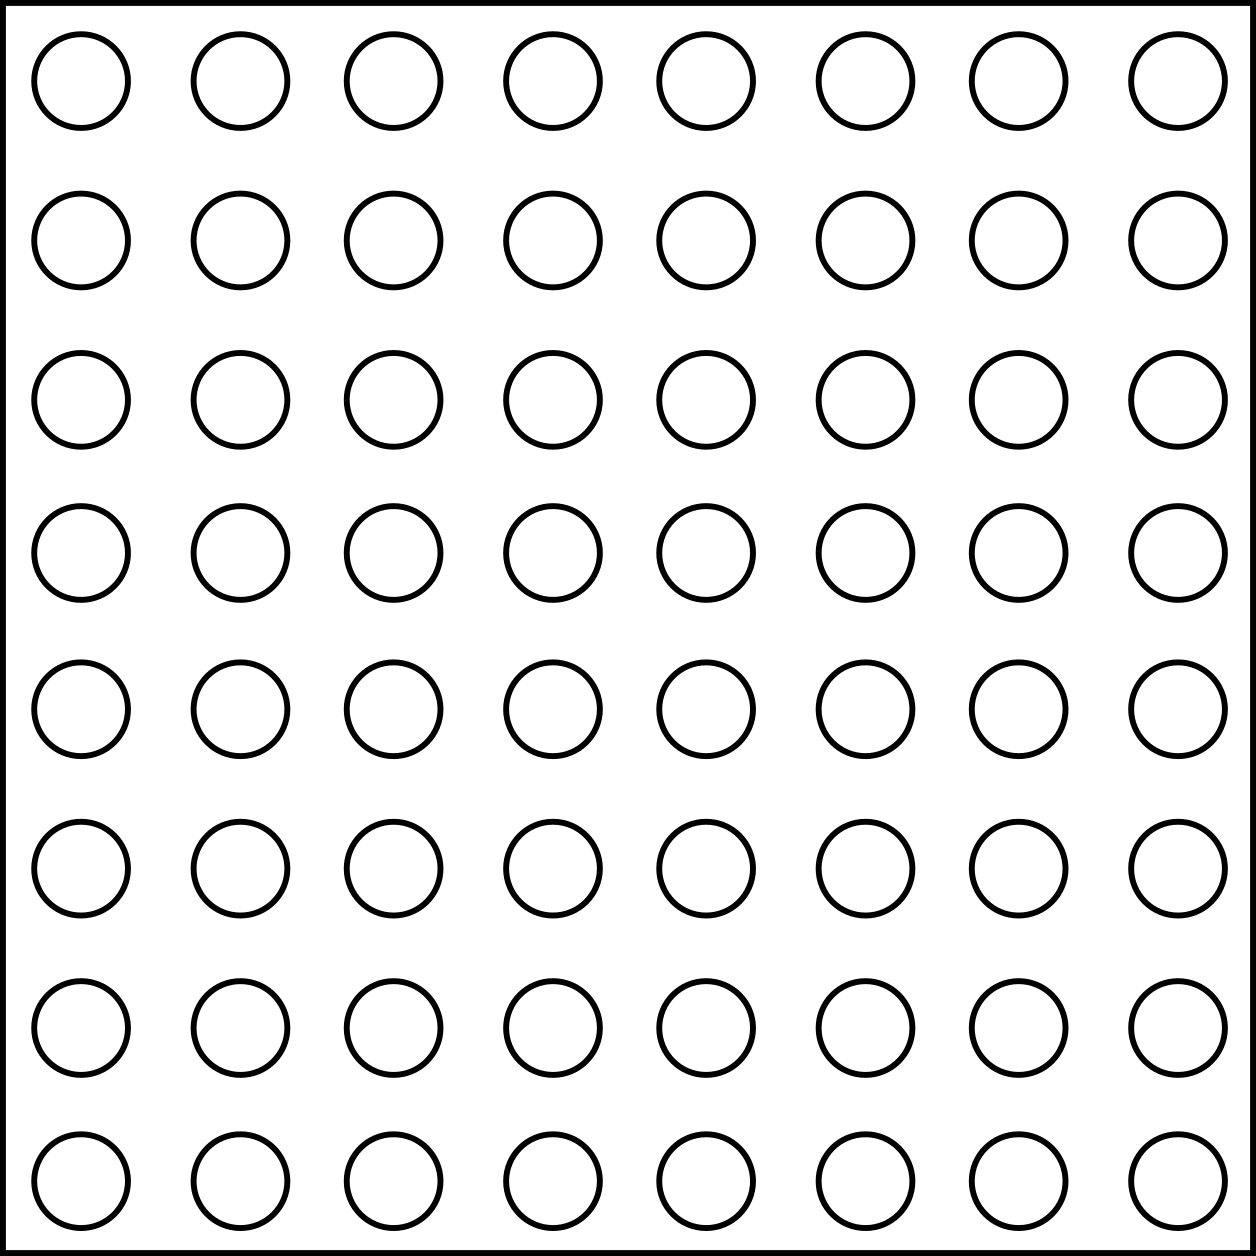
\includegraphics[width=0.80\textwidth]{cnn_neurones.png}

      \end{center}
    \end{column}

    \begin{column}<3->{0.33\textwidth}
      \begin{center}
        
\includegraphics[width=0.07\textwidth]{col.png}

      \end{center}
    \end{column}

  \end{columns}


\end{frame}


%%%%%%%%%%%%%%%%%%%%%%%%%%%%%%%%%%%%%%%%%%%%%%%%%%
\frame{
  \frametitle{Towards convolutional layers}

  \begin{columns}

    \begin{column}<1->{0.3\textwidth}
      \begin{center}
        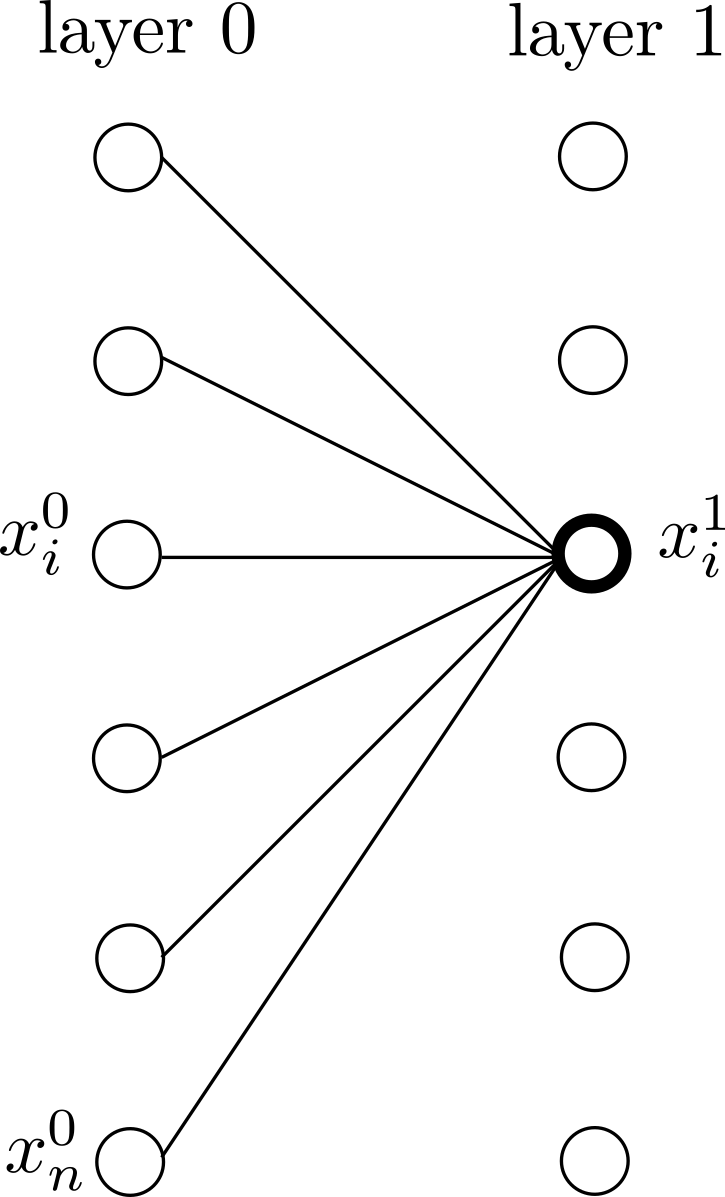
\includegraphics[width=0.74\textwidth]{fully_connected_layer.png}
        \\ \scriptsize{Fully connected layer: $n \times n$ weights and $n$ bias: $n(n+1)$ parameters}
      \end{center}
    \end{column}

    \begin{column}<2->{0.3\textwidth}
      \begin{center}
        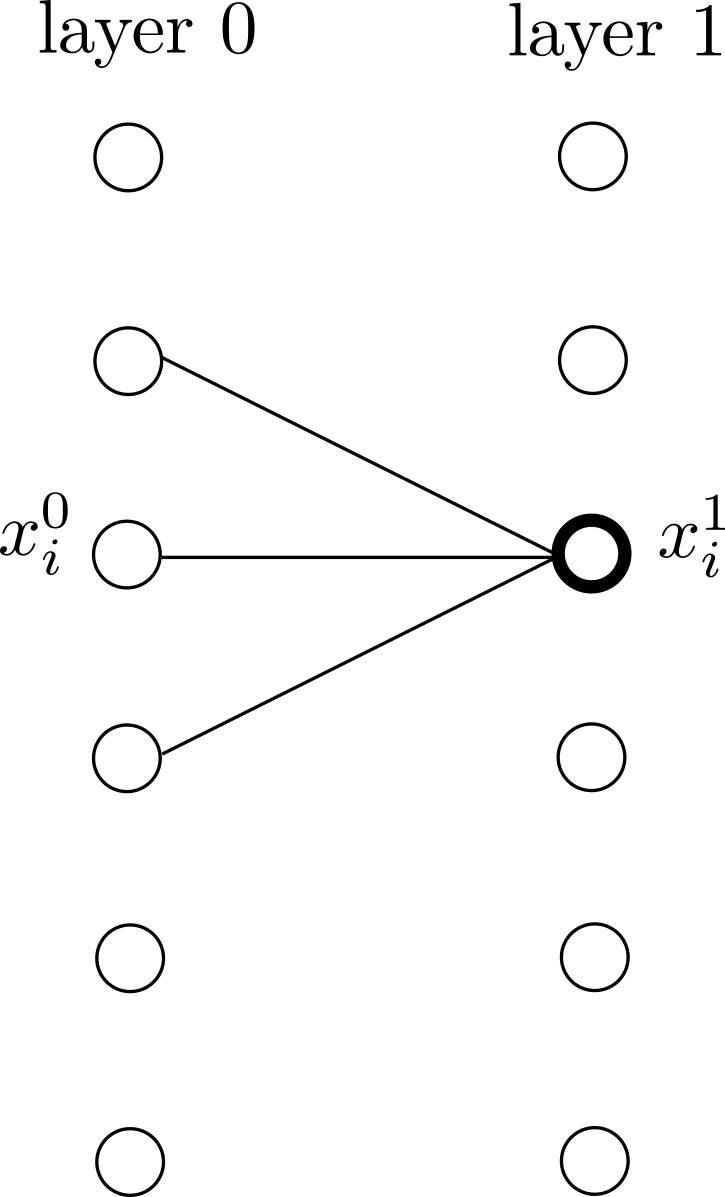
\includegraphics[width=0.74\textwidth]{locally_connected_layer.png}
        \\ \scriptsize{Locally conn. layer: $n(s+1)$ parameters}
      \end{center}
    \end{column}

    \begin{column}<3->{0.3\textwidth}
      \begin{center}
        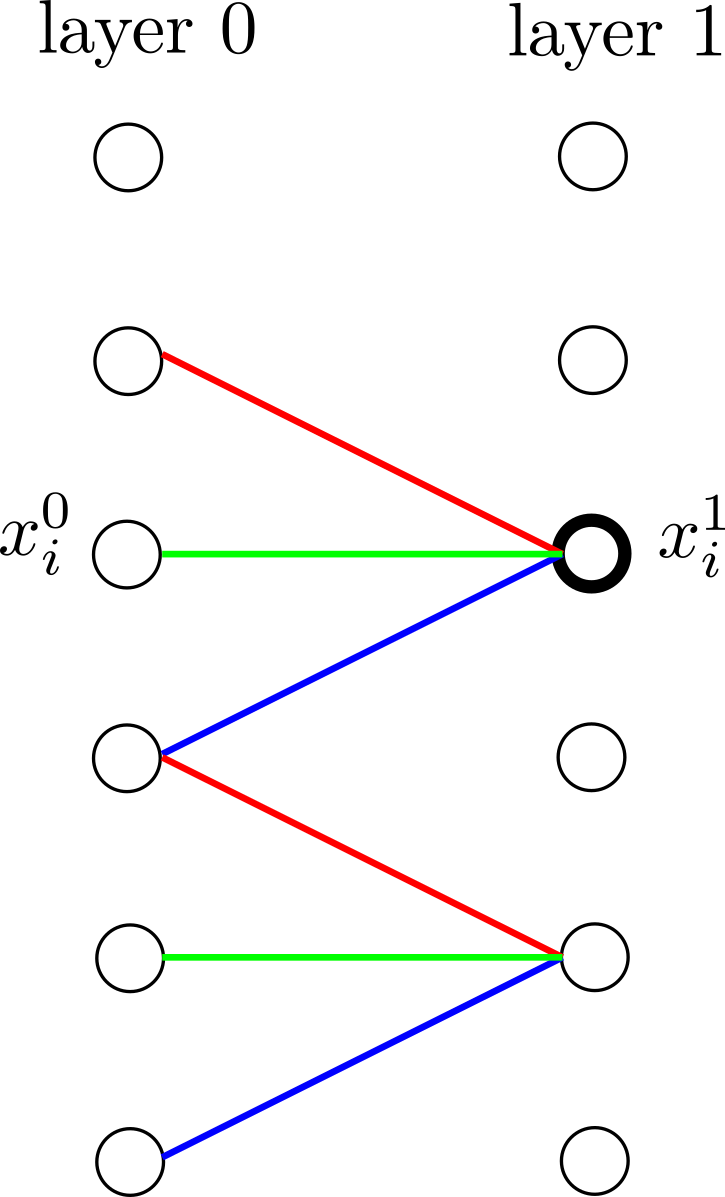
\includegraphics[width=0.74\textwidth]{convolutional_layer.png}
        \\ \scriptsize{Weight replication: $s+1$ parameters.\\
          \alert{Convolutional layer.}}
      \end{center}
    \end{column}

  \end{columns}


  \mode<beamer>{
  \begin{columns}
    \begin{column}<4->{.5\textwidth}
      Here, $s$ corresponds to number of incoming connections from the previous layer of a neuron. It is therefore equal to:

    \end{column}

    \begin{column}<5->{.5\textwidth}
      \begin{quizzblock}{}
      \begin{itemize}
      \item[1/] $3$
      \item[2/] $4$
      \item[3/] $9$
      \item[4/] $10$
      \end{itemize}

      \end{quizzblock}

    \end{column}
  \end{columns}
}
}

%%%%%%%%%%%%%%%%%%%%%%%%%%%%%%%%%%%%
\begin{frame}{Convolutional layer illustration in 2D}


  \begin{itemize}
  \item Illustration of a convolution of size $3 \times 3$
  \end{itemize}

  \begin{center}
    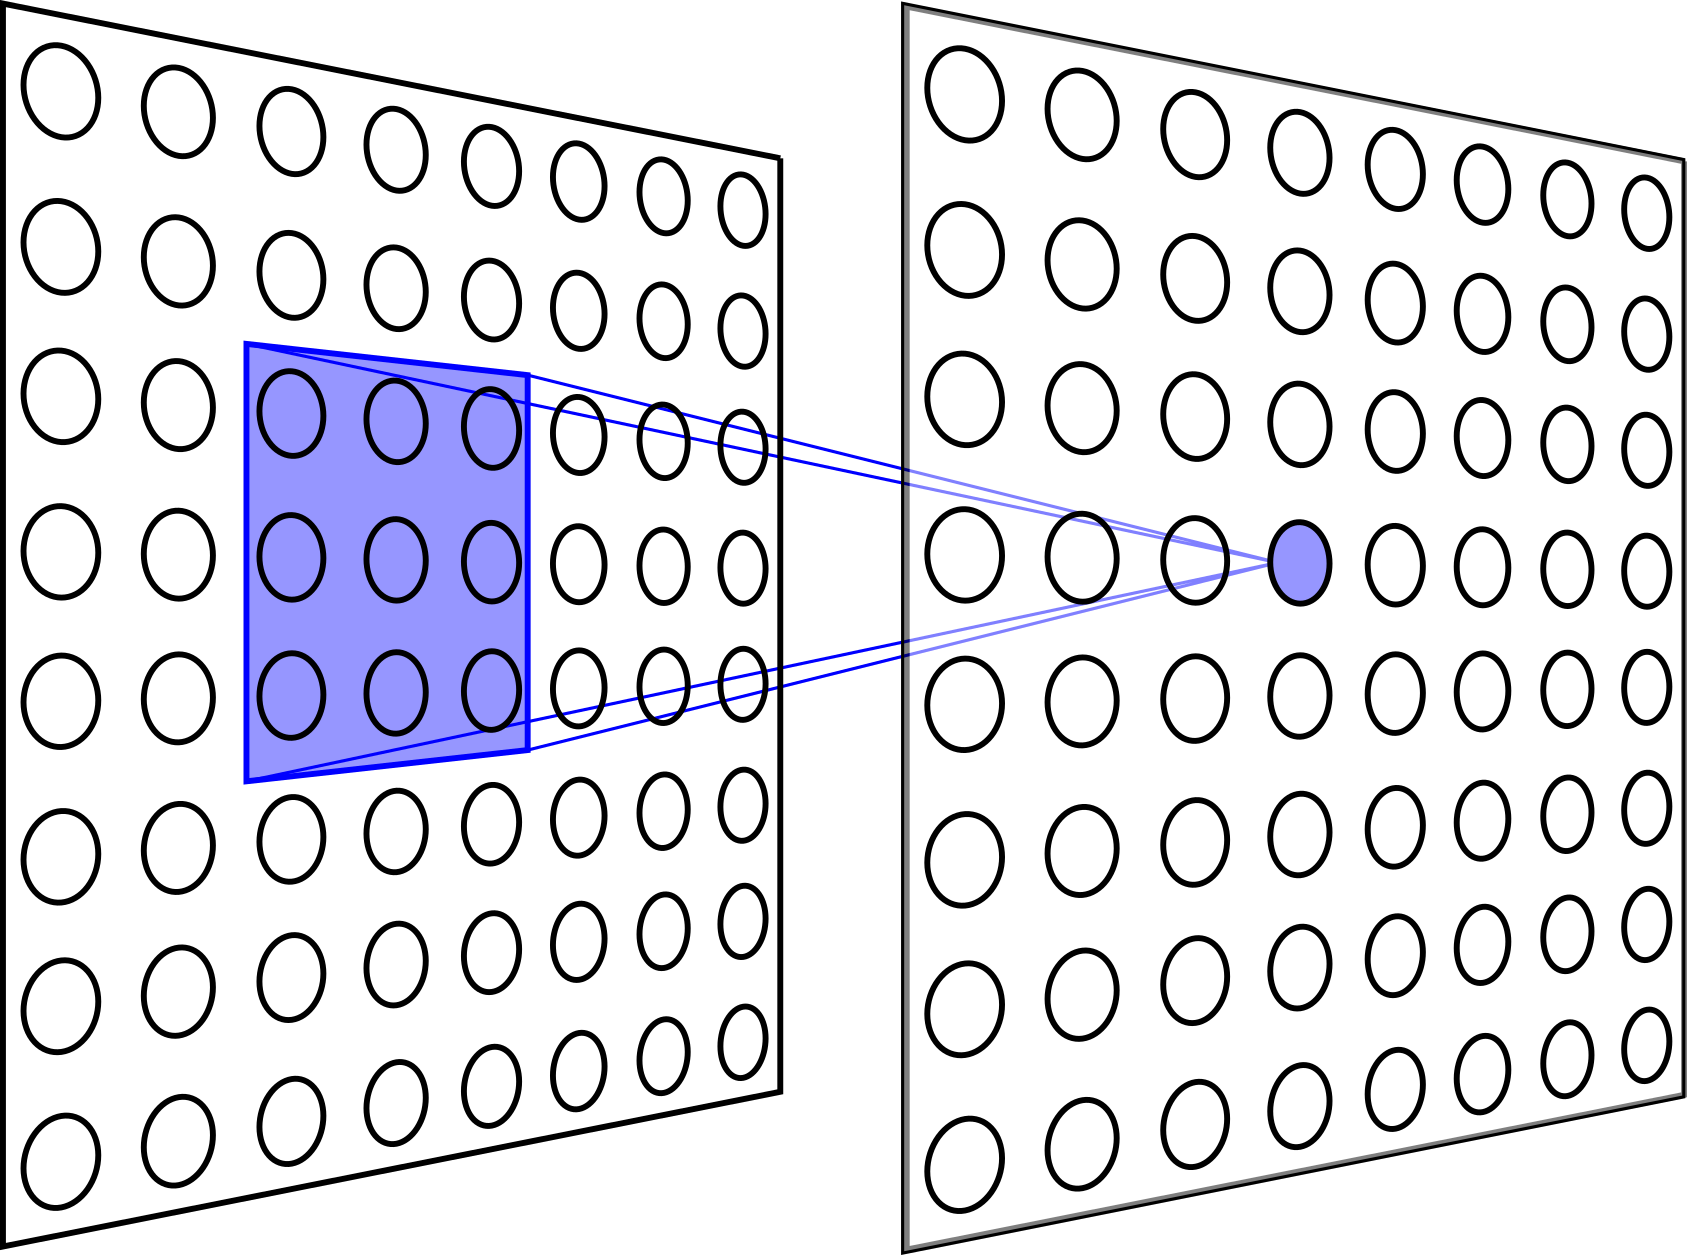
\includegraphics[width=0.5\textwidth]{cnn_complet}
  \end{center}


\end{frame}


%%%%%%%%%%%%%%%%%%%%%%%%%%%%%%%%%%%%%%%%%%%%%%%%%%
\frame{
  \frametitle{Convolutional layers: some figures}

  \begin{itemize}
  \item $3 \times 3$ convolutions: $s=9$
  \item \textcolor{blue}{Toy image: $n = 28 \times 28 = 784$}
  \item \textcolor{orange}{Typical image: $n = 1000 \times 1000 = 10^6$}
  \end{itemize}

  \begin{columns}

    \begin{column}{0.3\textwidth}
      \begin{center}
        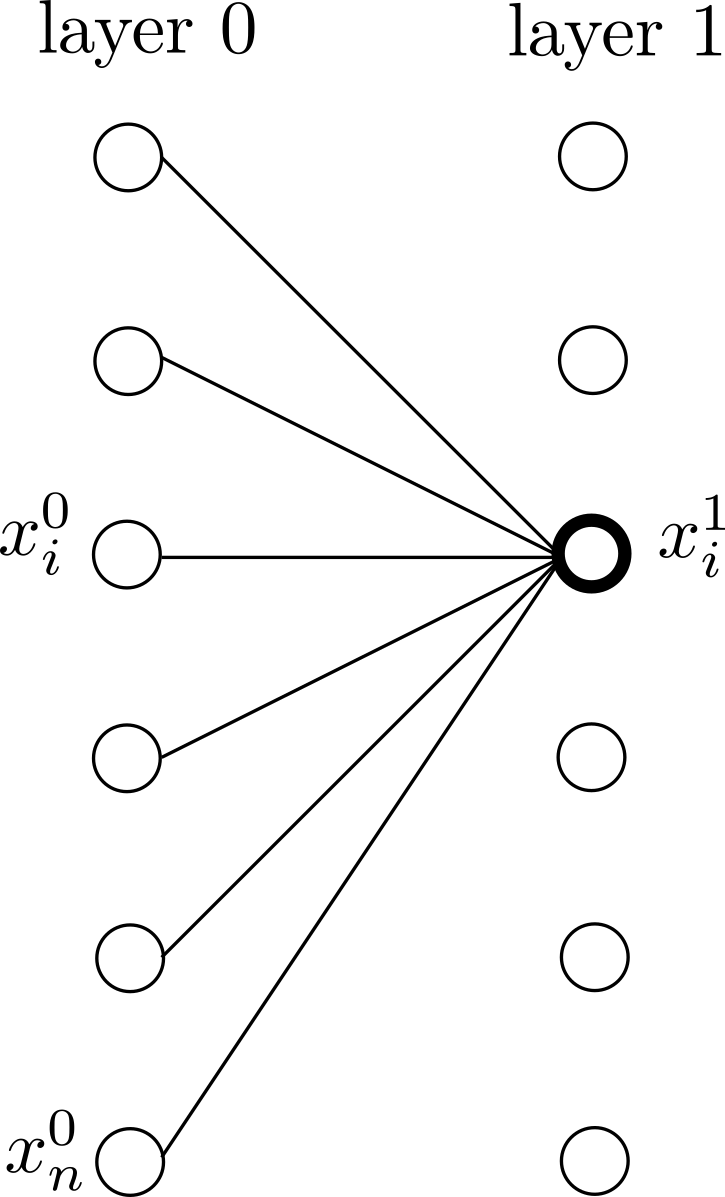
\includegraphics[width=0.74\textwidth]{fully_connected_layer.png}
        \\ \scriptsize{Fully connected layer: $n(n+1)$ parameters}
        \\ \textcolor{blue}{\scriptsize{$\approx 6.10^5$}}
        \\ \textcolor{orange}{\scriptsize{$\approx 10^{12}$}}
      \end{center}
    \end{column}

    \begin{column}{0.3\textwidth}
      \begin{center}
        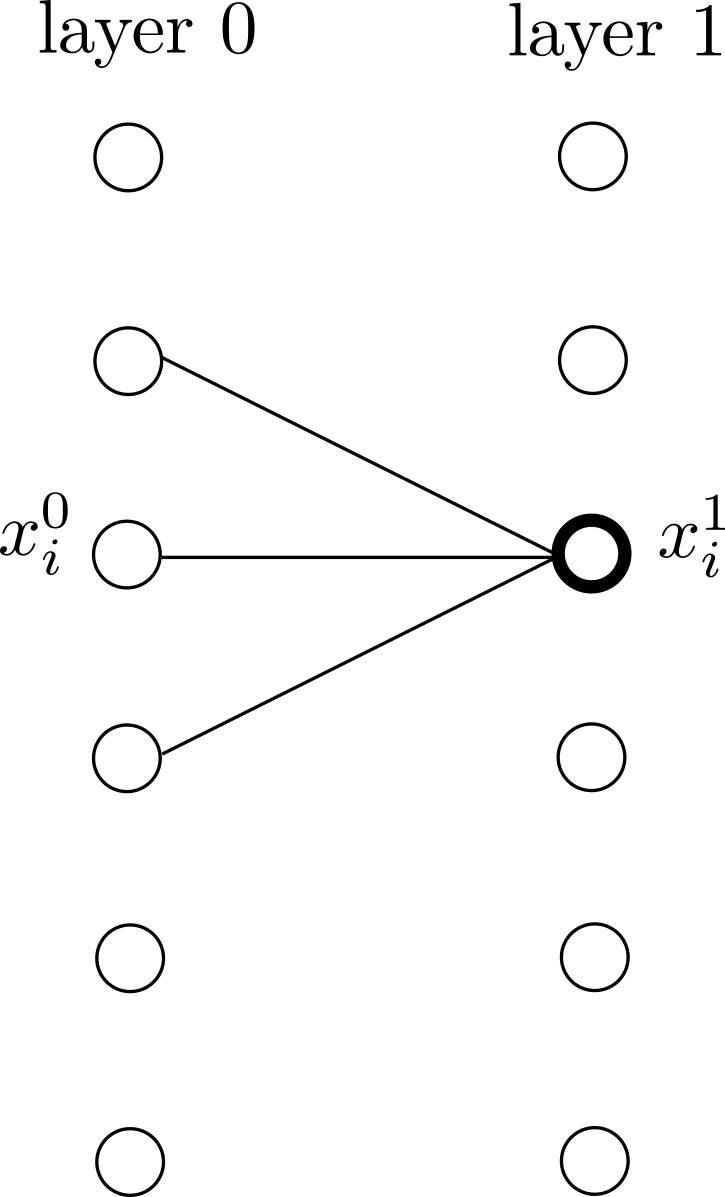
\includegraphics[width=0.74\textwidth]{locally_connected_layer.png}
        \\ \scriptsize{Locally conn. layer: $n(s+1)$ parameters}
        \\ \textcolor{blue}{\scriptsize{$7840$}}
        \\ \textcolor{orange}{\scriptsize{$10^7$}}
      \end{center}
    \end{column}

    \begin{column}{0.3\textwidth}
      \begin{center}
        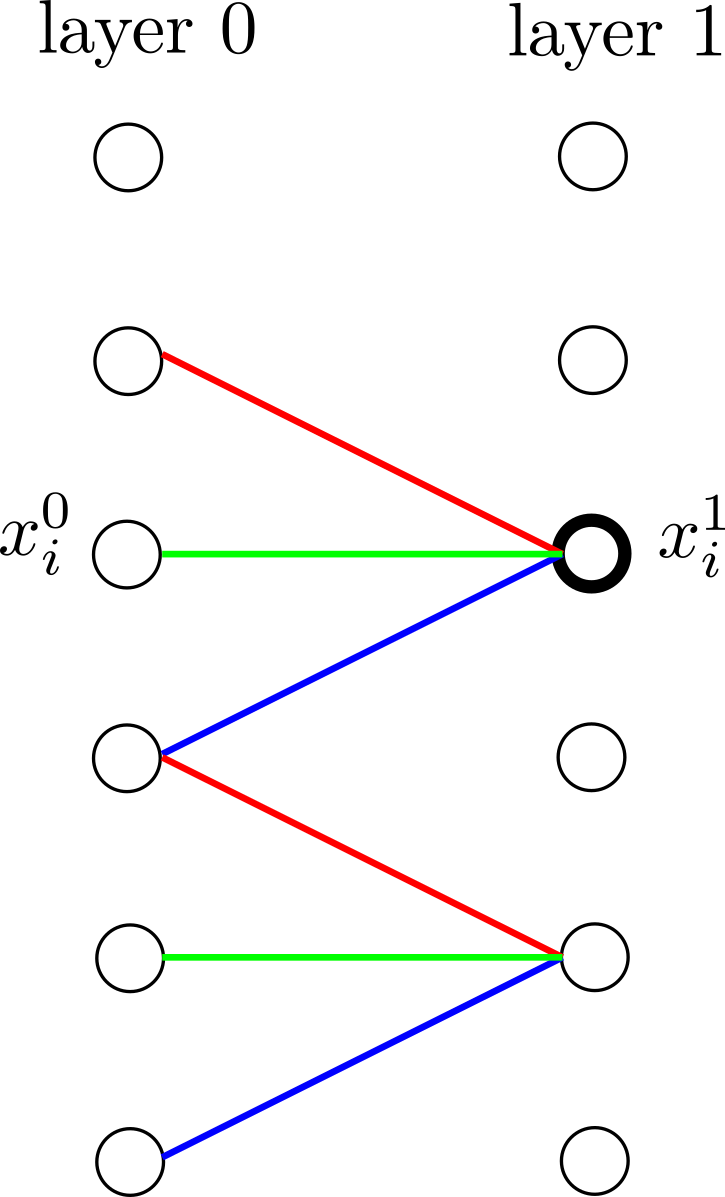
\includegraphics[width=0.74\textwidth]{convolutional_layer.png}
        \\ \scriptsize{Weight replication: $s+1$ parameters.}
        \\ \textcolor{blue}{\scriptsize{$10$}}
        \\ \textcolor{orange}{\scriptsize{$10$}}

      \end{center}
    \end{column}

  \end{columns}

  %% \begin{block}<4->{}
  %%   A convolutional layer computes a convolution, plus a constant, of the precedent layer.
  %% \end{block}


}

%%%%%%%%%%%%%%%%%%%%%%%%%%%%%%%%%%%%
\begin{frame}{Convolutional layers are fully connected layers}

  Convolutional layers are fully connected layers such that:
  \begin{itemize}
  \item the weights of all non-local connections are set to zero;
  \item the weights are shared among all the neurons of the same channel.
  \end{itemize}

  These limitations correspond to two inductive biases:

\begin{itemize}
\item local structure and
\item translation invariance.
\end{itemize}

  They make the network much more manageable (memory, optimization). Is the loss in generality important?

\end{frame}

%%%%%%%%%%%%%%%%%%%%%%%%%%%%%%%%%%%%
\begin{frame}{Dealing with borders}

  \begin{figure}
    \includegraphics[height=5cm]{conv_border_effect}
  \end{figure}

\end{frame}

%%%%%%%%%%%%%%%%%%%%%%%%%%%%%%%%%%%%
\begin{frame}{First solution: keep only well defined outputs}

\begin{columns}
  \begin{column}{.5\textwidth}
  \begin{figure}
    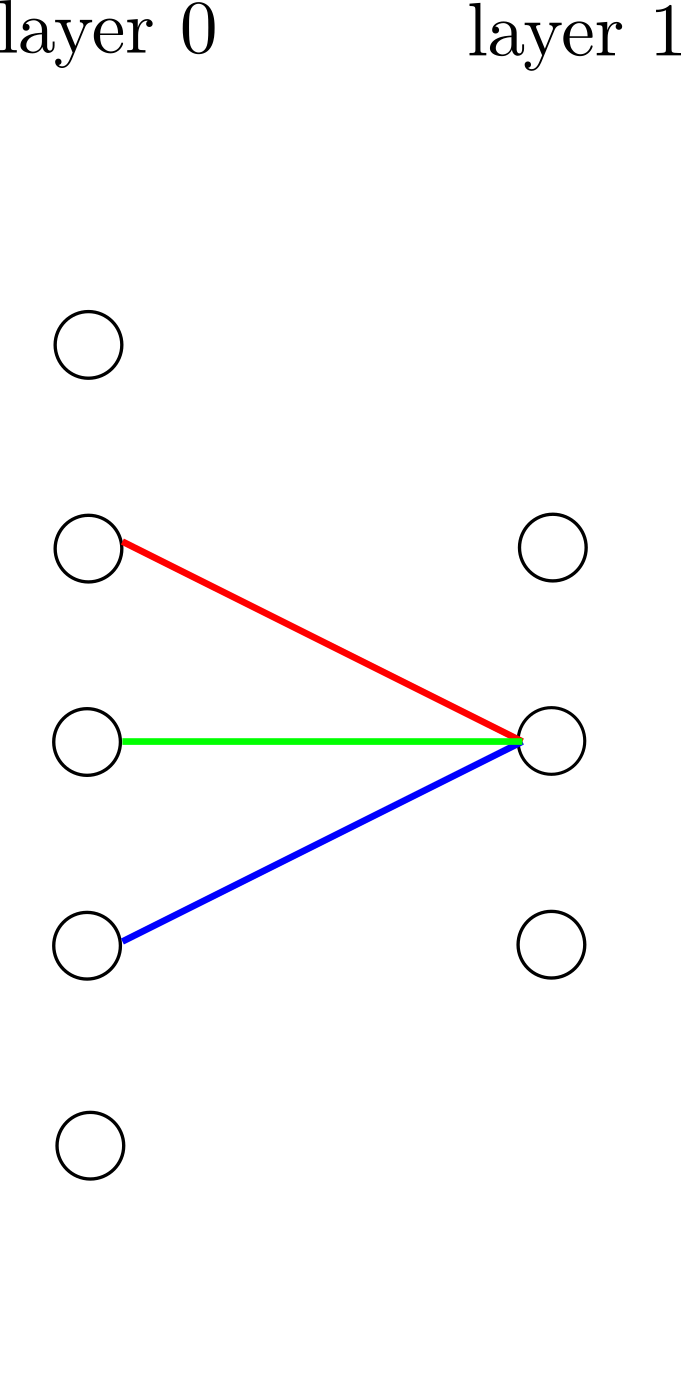
\includegraphics[height=5cm]{conv_border_effect2}
  \end{figure}

  \end{column}

  \begin{column}{.5\textwidth}
  \begin{itemize}
  \item Pros:
    \begin{itemize}
    \item border effect disappears
    \end{itemize}
  \item Cons:
    \begin{itemize}
    \item Lack of flexibility
    \item With deep networks, the field can become very small, or disappear
    \end{itemize}
  \end{itemize}

  \end{column}
\end{columns}



\end{frame}


%%%%%%%%%%%%%%%%%%%%%%%%%%%%%%%%%%%%
\begin{frame}{Second solution: zero padding}

\begin{columns}
  \begin{column}{.5\textwidth}
  \begin{figure}
    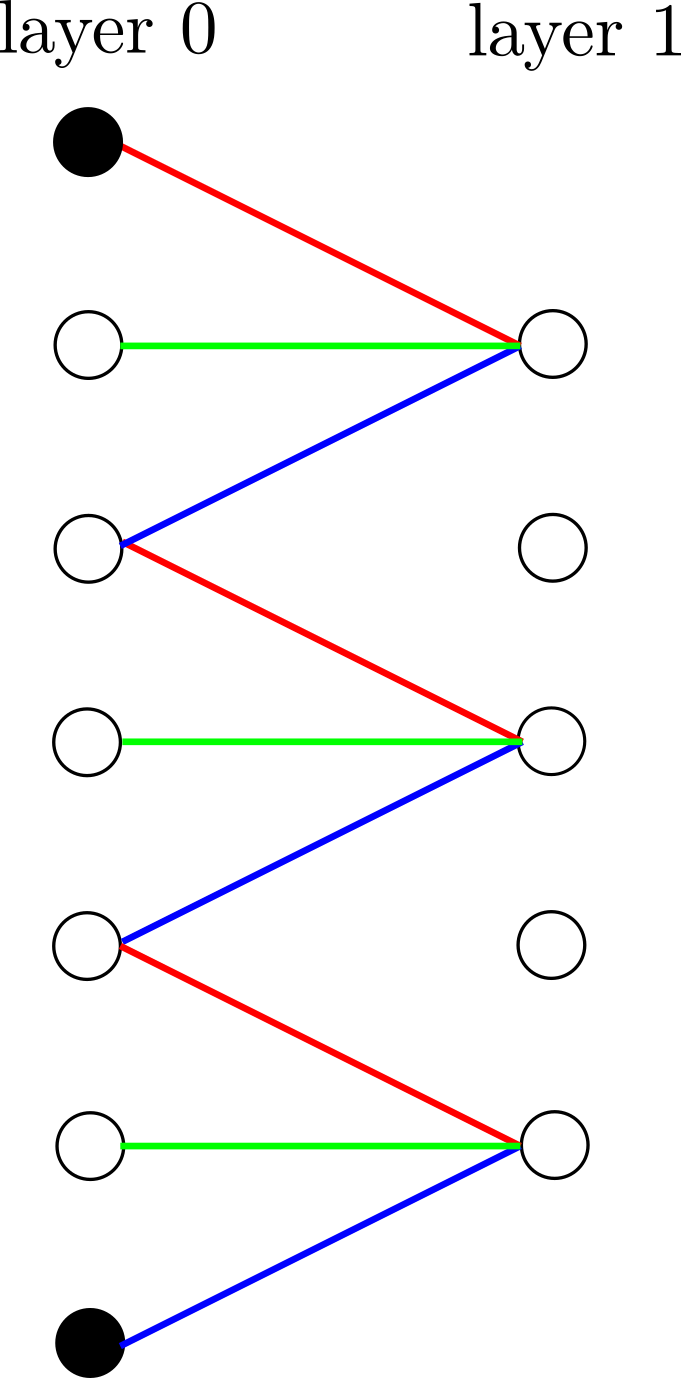
\includegraphics[height=5cm]{conv_border_effect3}
  \end{figure}
\end{column}

  \begin{column}{.5\textwidth}

  \begin{itemize}
  \item Pros:
    \begin{itemize}
    \item More flexible architecture
    \end{itemize}
  \item Cons:
    \begin{itemize}
    \item Border effect still present
    \end{itemize}
  \end{itemize}
  \end{column}
\end{columns}


\end{frame}





%%%%%%%%%%%%%%%%%%%%%%%%%%%%%%%%%%%%%%%%%%%%%%%%%%
\frame{
  \frametitle{Stride}

  A convolutional layer can at the same time downsample the image by applying a sampling step, or \emph{stride}.

  \begin{columns}

    \begin{column}<1->{0.3\textwidth}
      \begin{center}
        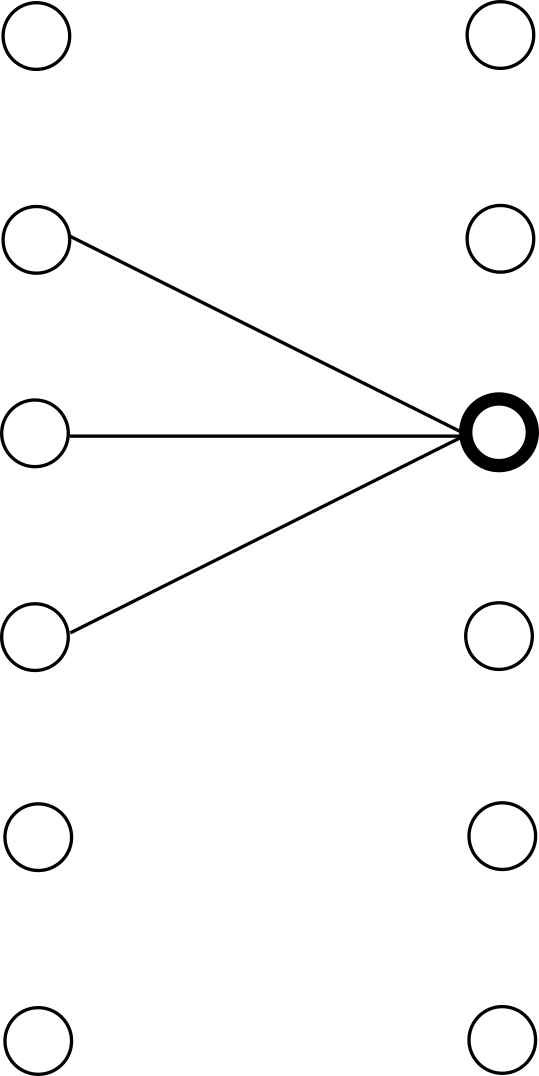
\includegraphics[width=0.60\textwidth]{stride1.png}
        \\ \scriptsize{Stride 1}
      \end{center}
    \end{column}

    \begin{column}<2->{0.3\textwidth}
      \begin{center}
        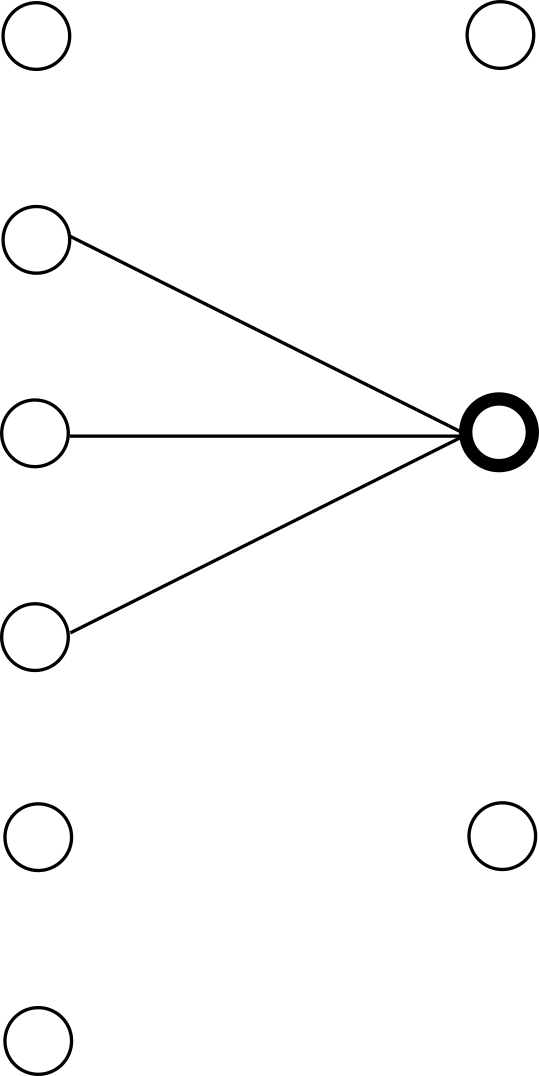
\includegraphics[width=0.60\textwidth]{stride2.png}
        \\ \scriptsize{Stride 2}
      \end{center}
    \end{column}

    \begin{column}<3>{0.3\textwidth}
      \begin{center}
        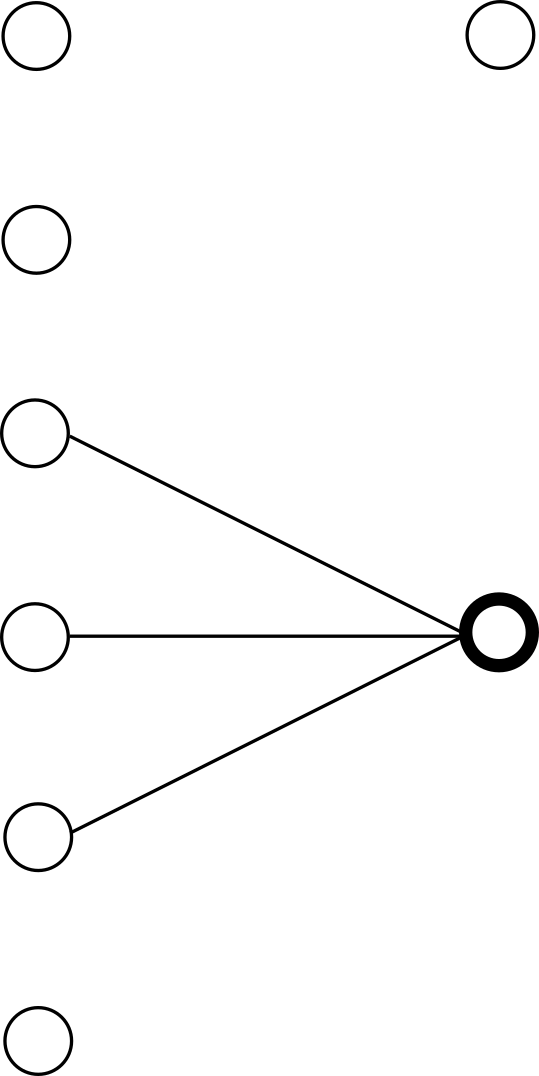
\includegraphics[width=0.60\textwidth]{stride3.png}
        \\ \scriptsize{Stride 3}
      \end{center}
    \end{column}

  \end{columns}

}

%%%%%%%%%%%%%%%%%%%%%%%%%%%%%%%%%%%%
\begin{frame}{Dilated convolutions}

  Dilated convolutions are used to increase the size of the \emph{receptive field} of the network.

  \begin{columns}

    \begin{column}<1->{0.3\textwidth}
      \begin{center}
        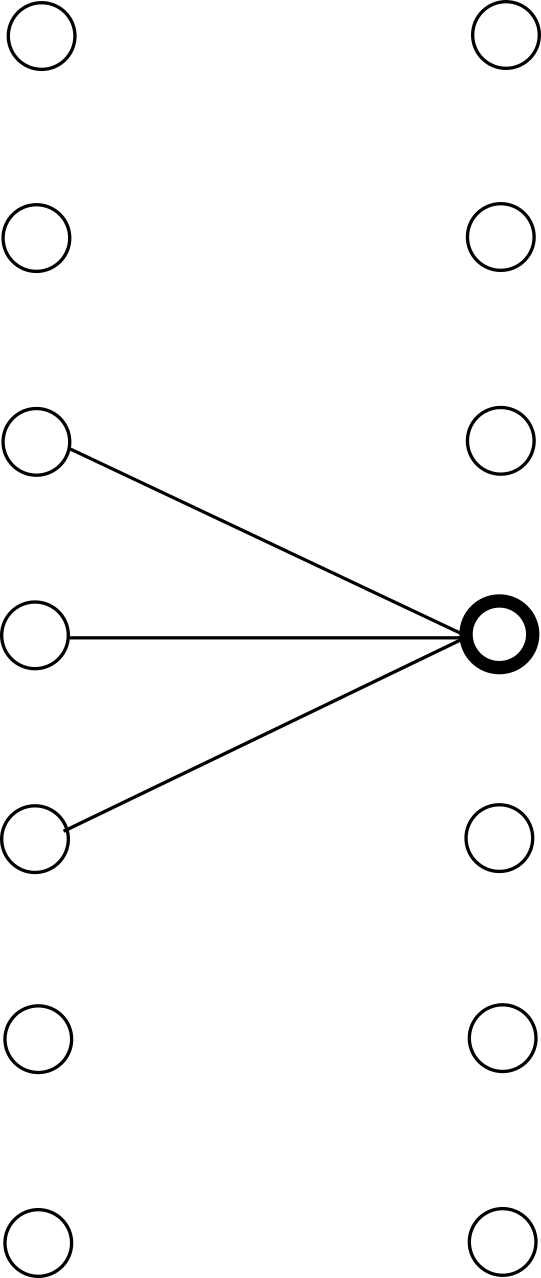
\includegraphics[width=0.60\textwidth]{dil_conv1.png}
        \\ \scriptsize{Normal convolution}
      \end{center}
    \end{column}

    \begin{column}<2->{0.3\textwidth}
      \begin{center}
        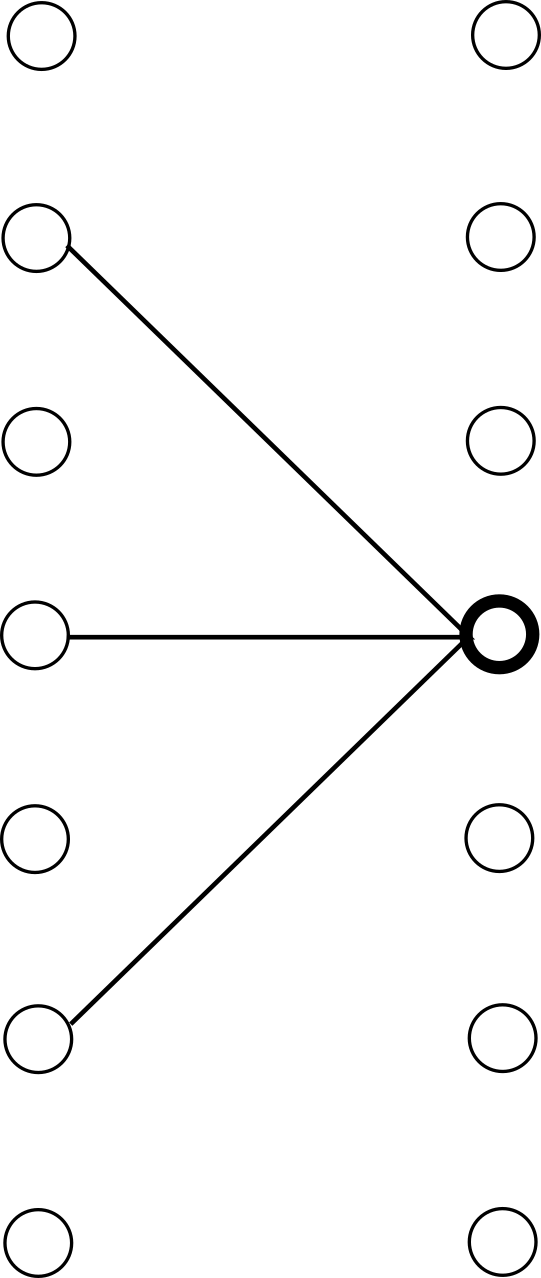
\includegraphics[width=0.60\textwidth]{dil_conv2.png}
        \\ \scriptsize{Dilation rate 2}
      \end{center}
    \end{column}

    \begin{column}<3->{0.3\textwidth}
      \begin{center}
        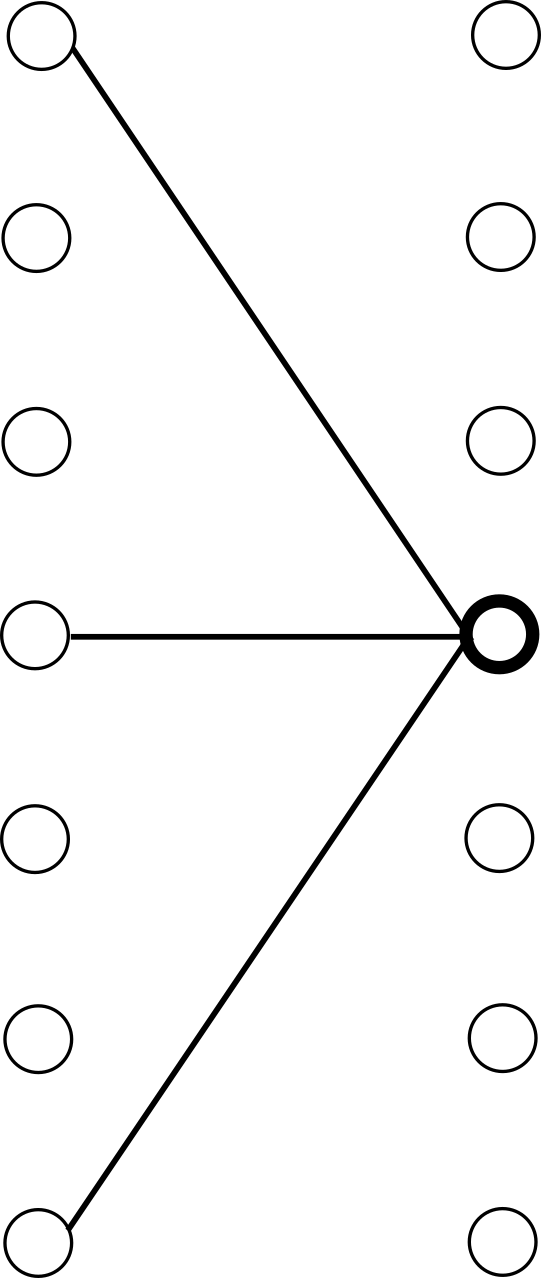
\includegraphics[width=0.60\textwidth]{dil_conv3.png}
        \\ \scriptsize{Dilation rate 3}
      \end{center}
    \end{column}


  \end{columns}


\end{frame}

%%%%%%%%%%%%%%%%%%%%%%%%%%%%%%%%%%%%%%%%%%%%%%%%%%
\frame{
  \frametitle{Several filters in the same convolutional layer}


  \begin{columns}
    \begin{column}{.53\textwidth}
      \begin{center}
        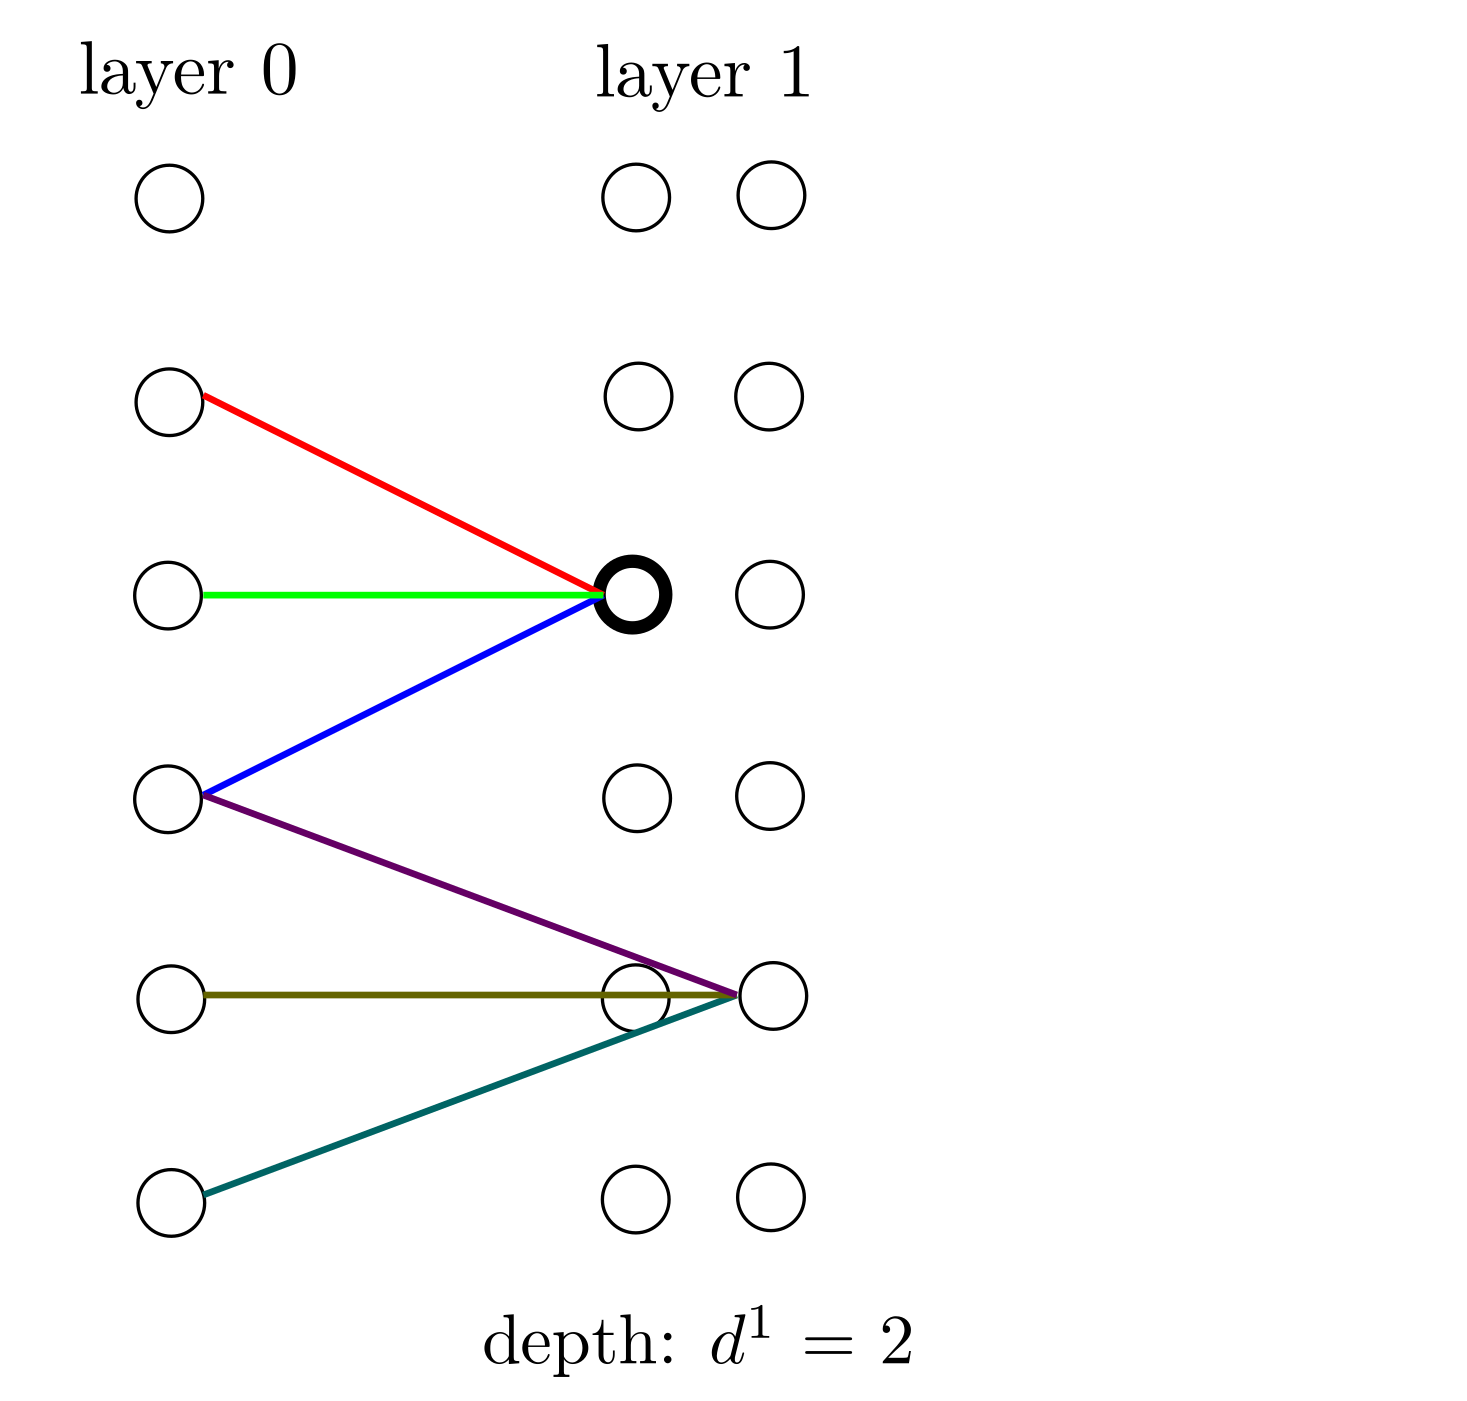
\includegraphics[width=\textwidth]{convolutional_layer2.png}
      \end{center}

    \end{column}

    \begin{column}{.47\textwidth}
      \begin{block}{Note on vocabulary}
        The filters are also called \alert{channels} or \alert{feature maps}.
      \end{block}
    \end{column}
  \end{columns}



}

%%%%%%%%%%%%%%%%%%%%%%%%%%%%%%%%%%%%%%%%%%%%%%%%%%
\frame{
  \frametitle{Several filters in the same convolutional layer}

  \begin{center}
    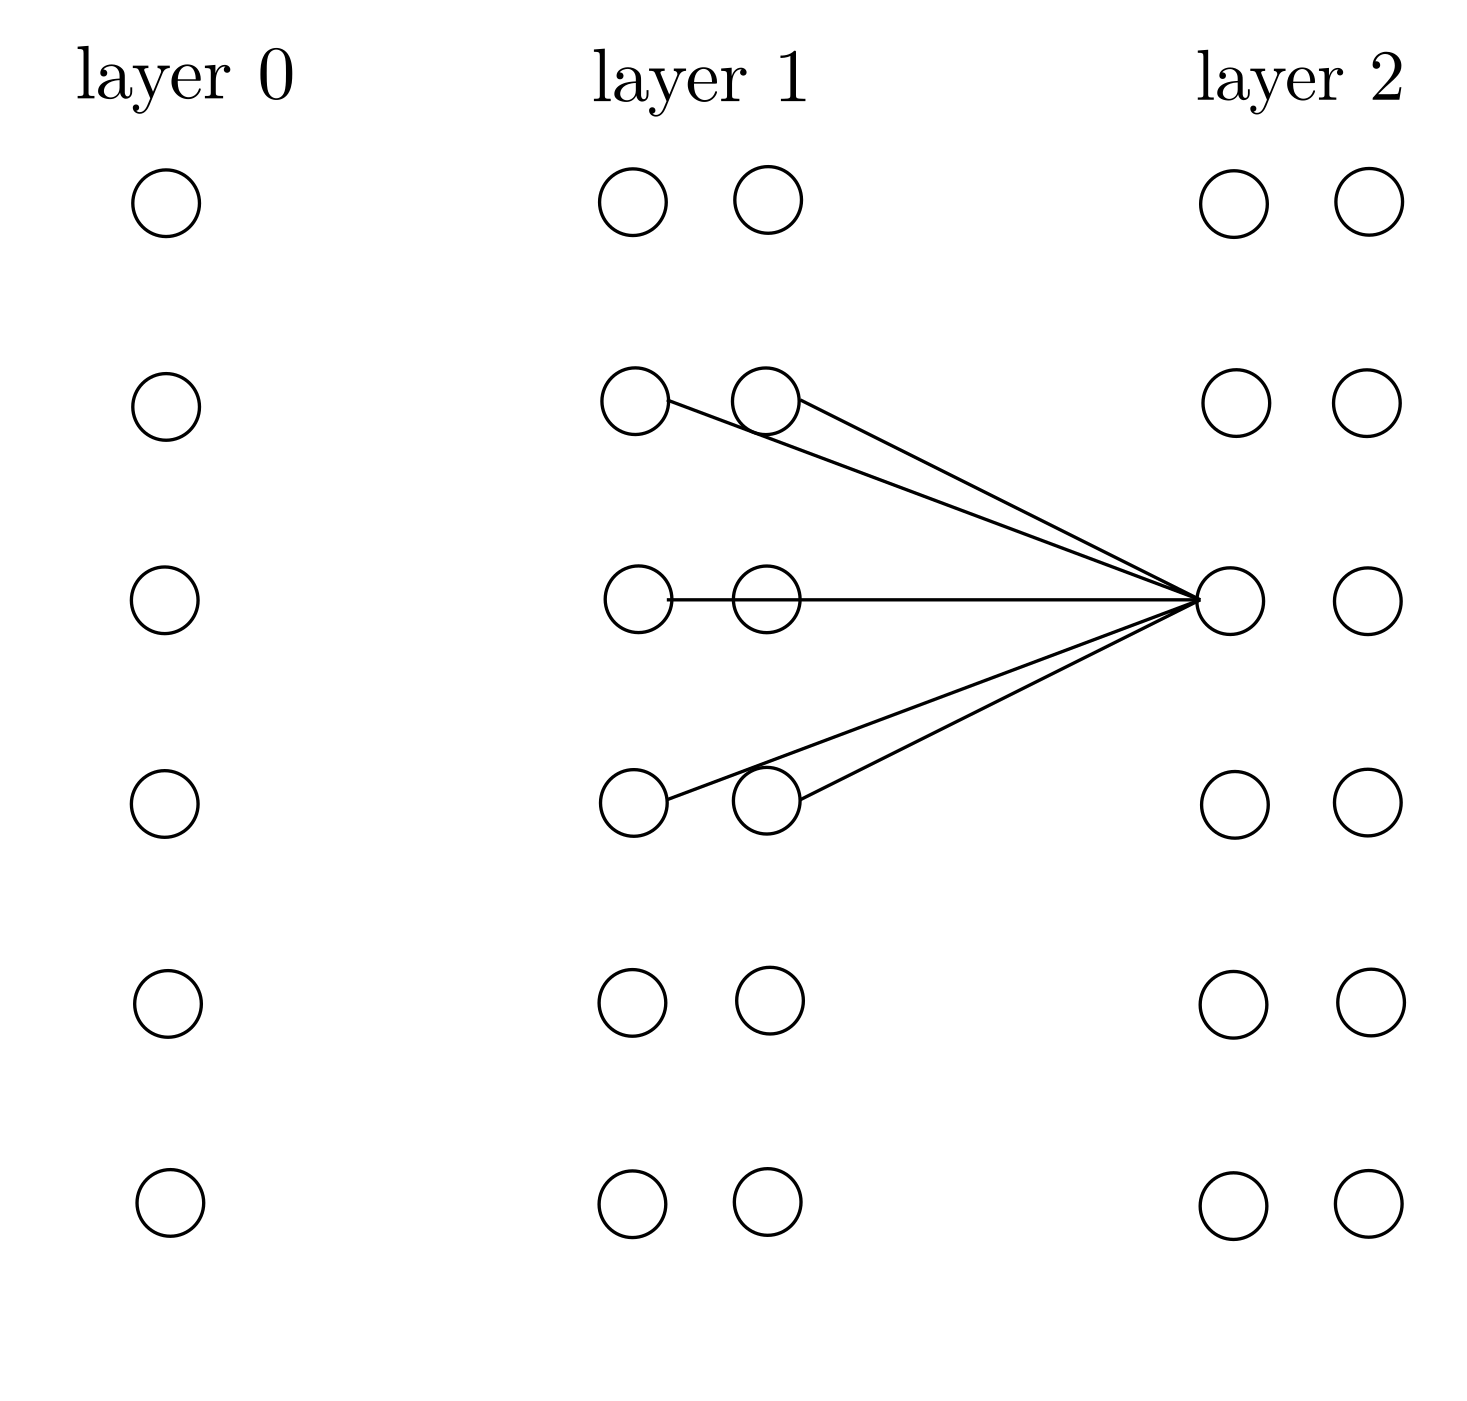
\includegraphics[width=0.53\textwidth]{convolutional_layer3.png}

  \end{center}

}

%%%%%%%%%%%%%%%%%%%%%%%%%%%%%%%%%%%%%%%%%%%%%%%%%%
\frame{
  \frametitle{Several filters in the same convolutional layer}

  \begin{center}
    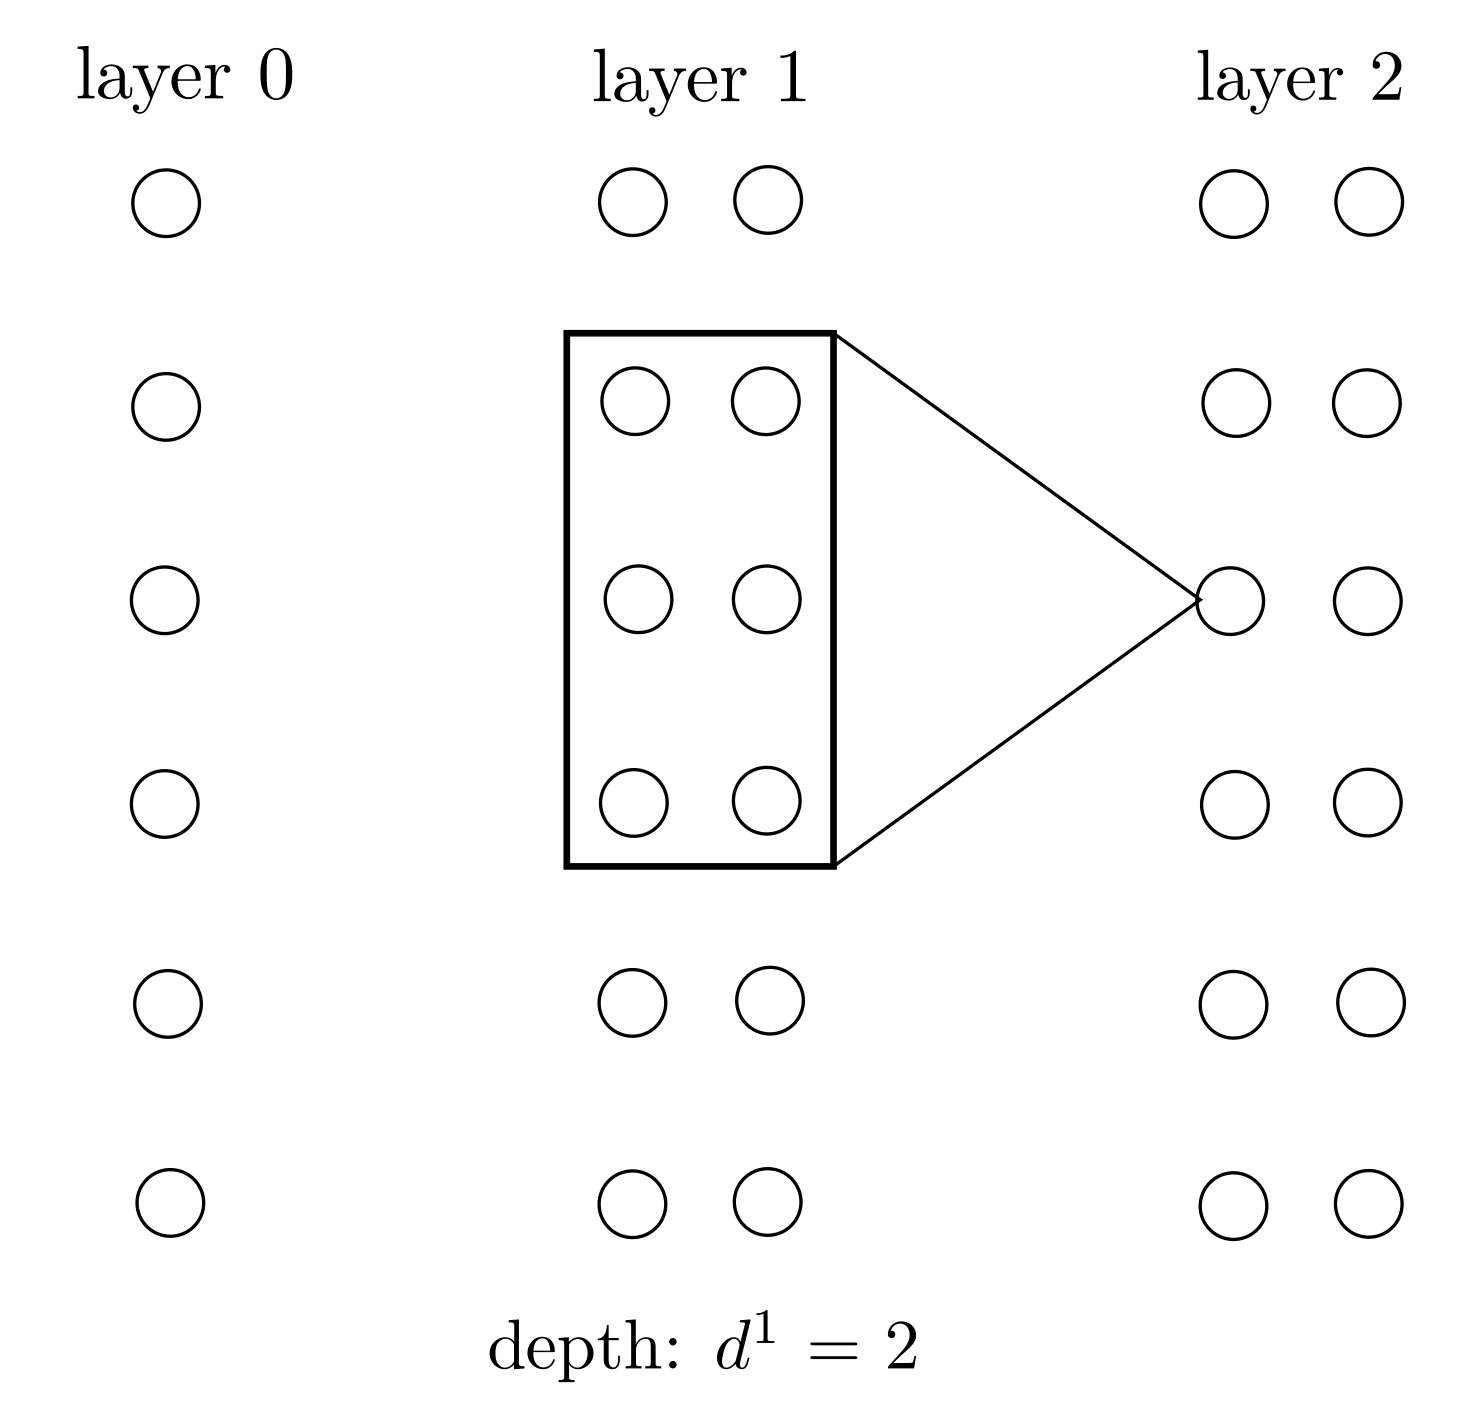
\includegraphics[width=0.53\textwidth]{convolutional_layer4.png}

  \end{center}


}

%%%%%%%%%%%%%%%%%%%%%%%%%%%%%%%%%%%%%%%%%%%%%%%%%%
\frame{
  \frametitle{Consequences on the parameter number}

  \begin{columns}
    \begin{column}{.5\textwidth}
      \begin{center}
        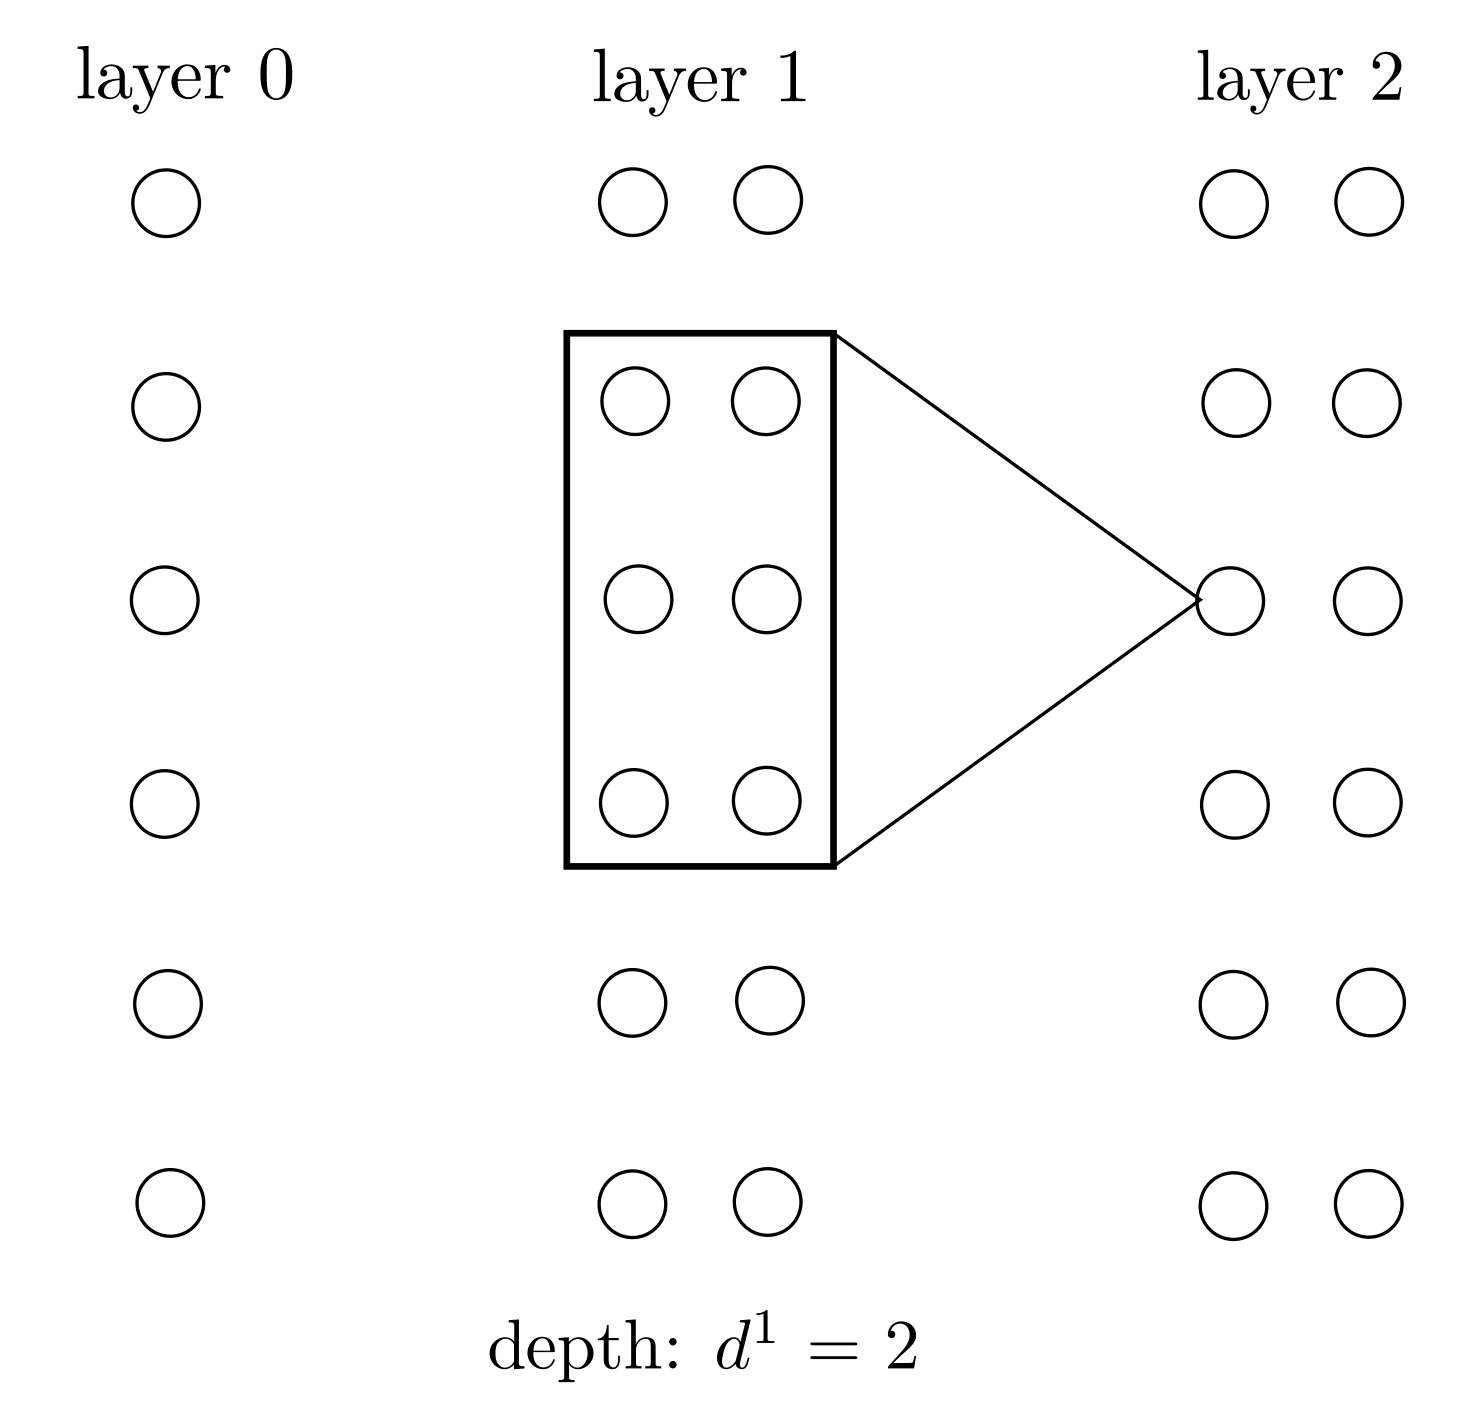
\includegraphics[width=\textwidth]{convolutional_layer4.png}
      \end{center}
    \end{column}

    \begin{column}{.5\textwidth}
      \begin{quizzblock}{How many parameters do we have in layer 1?}
        \begin{itemize}
        \item[1/] $c_1 \times (s + 1)$
        \item[2/] $c_1 \times s$
        \item[3/] $(c_1 + 1) \times s$
        \end{itemize}
      \end{quizzblock}
    \end{column}

  \end{columns}

}


%%%%%%%%%%%%%%%%%%%%%%%%%%%%%%%%%%%%%%%%%%%%%%%%%%
\frame{
  \frametitle{Consequences on the parameter number}

\begin{columns}
  \begin{column}{.5\textwidth}
  \begin{center}
    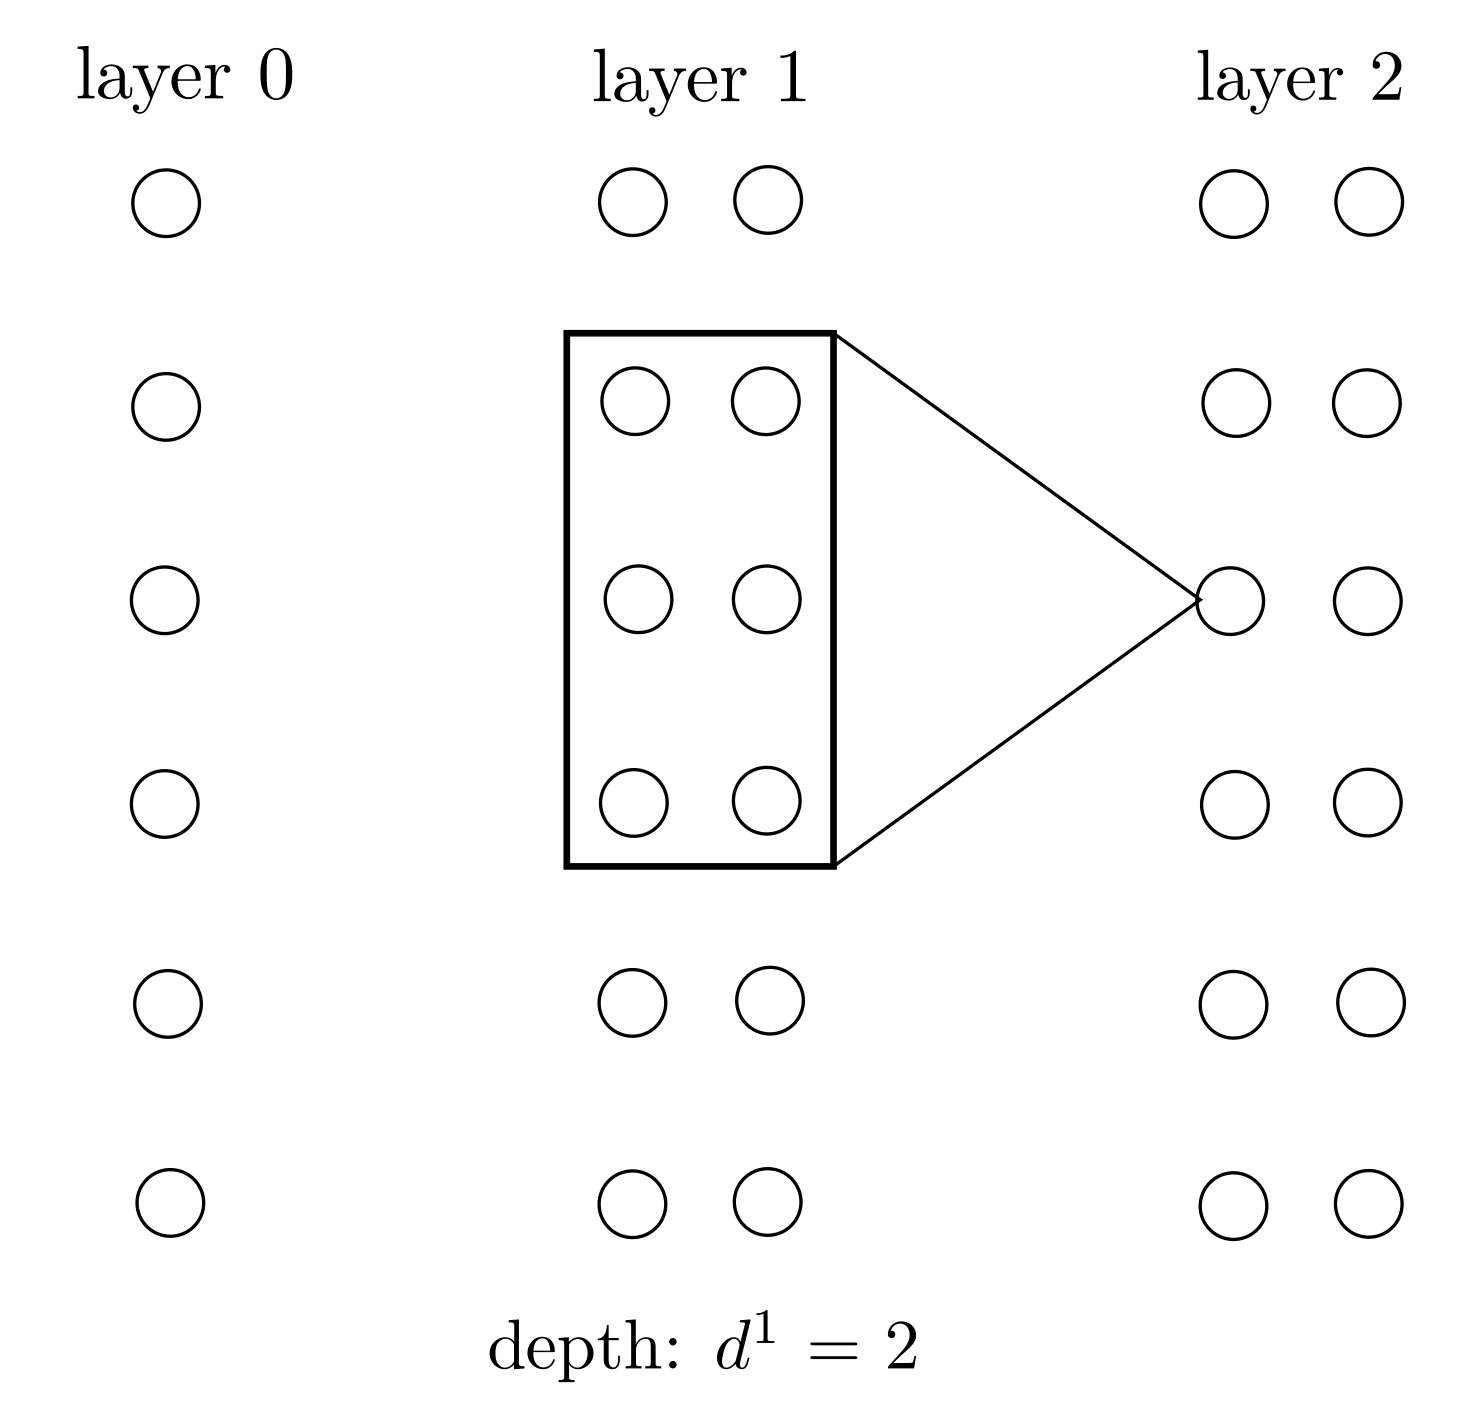
\includegraphics[width=\textwidth]{convolutional_layer4.png}
  \end{center}
  \end{column}

  \begin{column}{.5\textwidth}
  \begin{quizzblock}{How many parameters do we have in layer 2?}
    \begin{itemize}
    \item[1/] $c_2 \times c_1 \times s$
    \item[2/] $c_2 \times (c_1 \times s + 1)$
    \item[3/] $(c_2 + 1) \times (c_1 \times s + 1)$
    \end{itemize}
  \end{quizzblock}
  \end{column}
\end{columns}

}



%%%%%%%%%%%%%%%%%%%%%%%%%%%%%%%%%%%%%%%%%%%%%%%%%%
\frame{
  \frametitle{Multi-channel images}

  An input image with $p$ channels (for instance a colour image with 3 channels) can be represented by an input layer with $p$ channels/filters.

  \begin{center}
    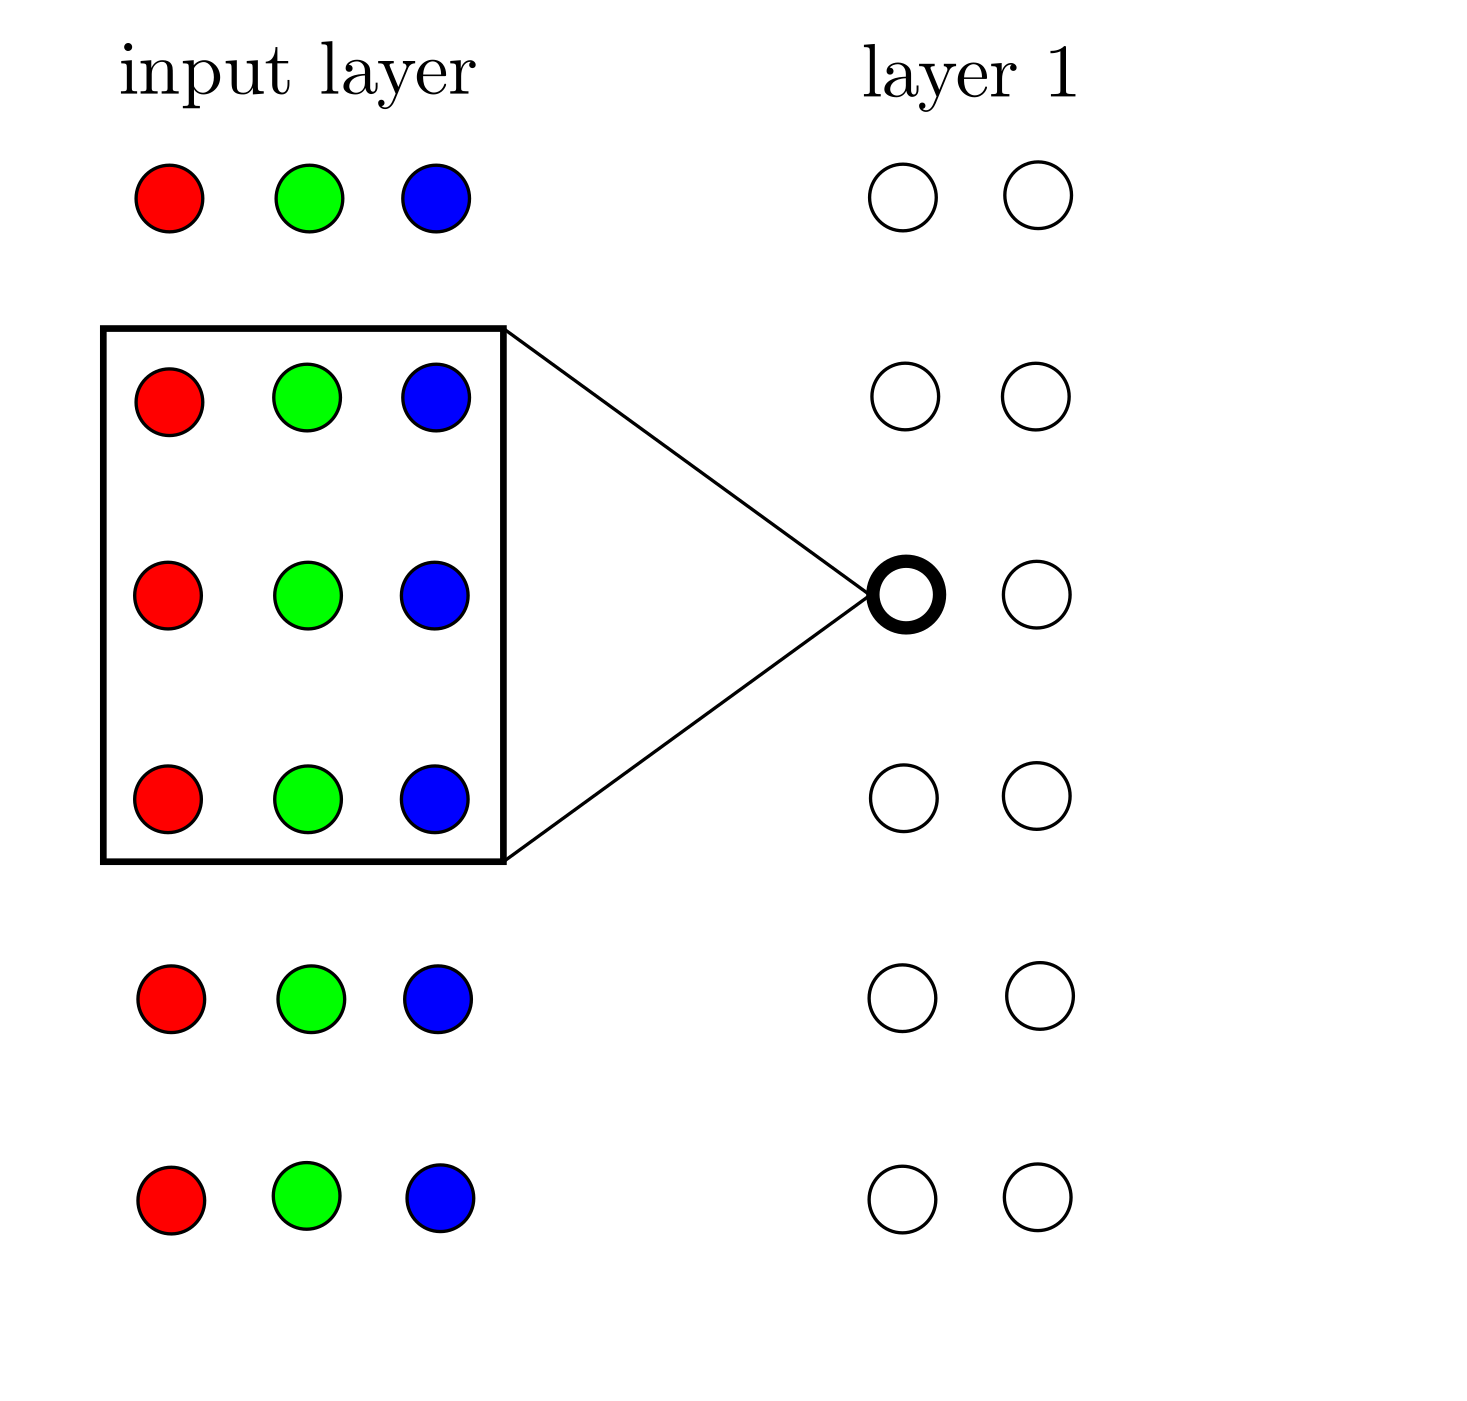
\includegraphics[height=0.51\textheight]{input_vector_image.png}
  \end{center}

}

%%%%%%%%%%%%%%%%%%%%%%%%%%%%%%%%%%%%
\begin{frame}{Depth-wise convolution}

  \begin{center}
    \includegraphics[height=0.51\textheight]{conv_depth_wise.png}
  \end{center}

  \begin{itemize}
  \item The previous layer must contain the same number of filters
  \item The number of parameters is drastically reduced
  \item These layers are interesting when combined with $1 \times 1$ convolutions...
  \end{itemize}


\end{frame}


%%%%%%%%%%%%%%%%%%%%%%%%%%%%%%%%%%%%
\begin{frame}{Dimension reduction}

  $1 \times 1$ convolutions are used to reduce the number of filters - this is called by some authors \emph{dimension reduction}.

  \begin{center}
    \includegraphics[height=0.51\textheight]{conv1x1.png}
  \end{center}

\end{frame}

%%%%%%%%%%%%%%%%%%%%%%%%%%%%%%%%%%%%
\begin{frame}{Decomposed convolution}

  The combination of depth-wise with $1 \times 1$ convolutions gives decomposed convolutions.

  \begin{center}
    \includegraphics[height=0.51\textheight]{conv_dec.png}
  \end{center}

  They are somehow a factorization of classical convolutions. Thus they allow reducing the number of parameters.

\end{frame}

%%%%%%%%%%%%%%%%%%%%%%%%%%%%%%%%%%%%
\begin{frame}{Decomposed convolution - number of parameters}
    \scriptsize

  \begin{center}
    \includegraphics[height=0.30\textheight]{conv_dec.png}
  \end{center}

  The input layer holds $c_1$ channels, and the output layer $c_2$. The size of the receptive field is $s$.

  \begin{columns}
  \begin{column}{.5\textwidth}

    \begin{quizzblock}{}
    How many parameters does the corresponding decomposed convolution layer contain?

\begin{enumerate}
\item $c_1 \times (s + 1) + c_2 \times (c_1 + 1)$
\item $c_1 \times s + c_2 \times c_1 $
\item $(c_1 + 1) \times s  + (c_2 + 1) \times c_1 $
\end{enumerate}

    \end{quizzblock}

  \end{column}

  \begin{column}{.5\textwidth}

    \begin{quizzblock}{}
How many parameters would the corresponding convolutional layer contain?

\begin{enumerate}
\item $c_1 \times s  \times c_2$
\item $(c_1 \times s + 1) \times (c_2 + 1)$
\item $(c_1 \times s + 1) \times c_2$
\end{enumerate}

    \end{quizzblock}

  \end{column}
\end{columns}



\end{frame}

%%%%%%%%%%%%%%%%%%%%%%%%%%%%%%%%%%%%
\begin{frame}<beamer>{Decomposed convolution - number of parameters}
    \scriptsize

  \begin{center}
    \includegraphics[height=0.30\textheight]{conv_dec.png}
  \end{center}

  The input layer holds $c_1$ channels, and the output layer $c_2$. The size of the receptive field is $s$.

  \begin{columns}
  \begin{column}{.5\textwidth}

    \begin{quizzblock}{}
    How many parameters does the corresponding decomposed convolution layer contain?

\begin{enumerate}
\item \alert{$c_1 \times (s + 1) + c_2 \times (c_1 + 1)$}
\item $c_1 \times s + c_2 \times c_1 $
\item $(c_1 + 1) \times s  + (c_2 + 1) \times c_1 $
\end{enumerate}

    \end{quizzblock}

  \end{column}

  \begin{column}{.5\textwidth}

    \begin{quizzblock}{}
How many parameters would the corresponding convolutional layer contain?

\begin{enumerate}
\item $c_1 \times s  \times c_2$
\item $(c_1 \times s + 1) \times (c_2 + 1)$
\item \alert{$(c_1 \times s + 1) \times c_2$}
\end{enumerate}

    \end{quizzblock}

  \end{column}
\end{columns}



\end{frame}



%%%%%%%%%%%%%%%%%%%%%%%%%%%%%%%%%%%%%%%%%%%%%%%%%%
%%%%%%%%%%%%%%%%%%%%%%%%%%%%%%%%%%%%%%%%%%%%%%%%%%
\section{Building convolutional networks}

%%%%%%%%%%%%%%%%%%%%%%%%%%%%%%%%%%%%%%%%%%%%%%%%%%

\frame{
  \frametitle{Max pooling}

  \begin{itemize}
  \item Convolutional networks often contain subsampling steps. A common way of doing this today is by using \emph{max pooling} layers with stride 2.

  \item Sampling is only applied along the spatial dimensions, not along the dimension of the filters.

  \end{itemize}

  \begin{center}
    \includegraphics[width=0.41\textwidth]{max_pooling.png}
  \end{center}

  \pause

  Note however a current trend that consists in using convolutional layers with a stride of 2

}



%%%%%%%%%%%%%%%%%%%%%%%%%%%%%%%%%%%%
\begin{frame}{Branch merging: concatenation}

  \begin{center}
    \includegraphics[width=0.5\textwidth]{concatenation.png}
  \end{center}

\end{frame}


%%%%%%%%%%%%%%%%%%%%%%%%%%%%%%%%%%%%
\begin{frame}{Branch merging: addition}

  \begin{center}
    \includegraphics[width=0.5\textwidth]{addition.png}
  \end{center}

\end{frame}

%%%%%%%%%%%%%%%%%%%%%%%%%%%%%%%%%%%%
\begin{frame}{Flatten}

  \begin{itemize}
  \item Transforms an array into a vector
  \item Loss of local structure
  \item This is typically done to transition between a convolutional layer and a fully-connected one.
  \end{itemize}

\end{frame}



%%%%%%%%%%%%%%%%%%%%%%%%%%%%%%%%%%%%
%% \begin{frame}{Branch merging}

%% \begin{columns}
%%   \begin{column}{.5\textwidth}
%%   \begin{center}
%%     \includegraphics[width=\textwidth]{concatenation.png}
%%     \\ Concatenation
%%   \end{center}

%%   \end{column}

%%   \begin{column}{.5\textwidth}
%%   \begin{center}
%%     \includegraphics[width=\textwidth]{addition.png}
%%     \\ Addition
%%   \end{center}

%%   \end{column}
%% \end{columns}

%% \end{frame}

%% %%%%%%%%%%%%%%%%%%%%%%%%%%%%%%%%%%%%
%% \begin{frame}{Skip connections}

%% \end{frame}
%%%%%%%%%%%%%%%%%%%%%%%%%%%%%%%%%%%%%%%%%%%%%%%%%%

\frame{
  \frametitle{Main components of a convolutional neural network}

  Many successful architectures, especially for image classification, follow the same pattern:

  \begin{enumerate}
  \item Several iterations of: One or several convolutional layers, with increasing depth, followed by max pooling
  \item A few fully connected layers
  \end{enumerate}

}

%%%%%%%%%%%%%%%%%%%%%%%%%%%%%%%%%%%%
\begin{frame}{2D representations}

  \centering
  \includegraphics[width=\textwidth]{fovea_convnet2}

  \vspace{1em}
  \pause

  \begin{columns}
    \begin{column}{.5\textwidth}
      \includegraphics[width=0.8\textwidth]{Fundus_photograph_of_normal_right_eye.jpg}
    \end{column}
    \begin{column}{.5\textwidth}
      This NN was used to estimate the position of the center of the macula on fundus images.
    \end{column}
  \end{columns}

  \source{NN is work of Robin Alais et al.\\Fundus image by Mikael Häggström, used with permission (CC0).}


\end{frame}

%%%%%%%%%%%%%%%%%%%%%%%%%%%%%%%%%%%%
\begin{frame}{3D representations}

  \begin{center}
    \begin{figure}
      \includegraphics[width=0.75\textwidth]{vgg16.png}
      \source{VGG16 (From https://www.cs.toronto.edu/~frossard/post/vgg16/)}
    \end{figure}
  \end{center}

\end{frame}


%% %%%%%%%%%%%%%%%%%%%%%%%%%%%%%%%%%%%%%%%%%%%%%%%%%%

%% \frame{
%% \frametitle{Example networks: fovea detection}

%%   \begin{center}
%%   \includegraphics[width=\textwidth]{fovea_convnet2.png}
%% \end{center}

%%   }

%%%%%%%%%%%%%%%%%%%%%%%%%%%%%%%%%%%%%%%%%%%%%%%%%%

%% \frame{
%% \frametitle{A typical convolutional architecture for image classification}

%% \begin{figure}
%%   \includegraphics[width=9.5cm]{conv_net_classif}
%%   \caption{Architecture used for the classification of the NORB dataset (from \cite{scherer_evaluation_2010})}
%% \end{figure}

%% Note that layer P4 can be seen as made of features, which are then classified by the two fully connected layers.


%% }

%%%%%%%%%%%%%%%%%%%%%%%%%%%%%%%%%%%%
\frame{
  \frametitle{Convolutional neural networks in deep learning}

  \begin{itemize}

    %% \item They play a major role in deep learning
  \item They are pivotal to many of the successes achieved by neural networks these recent years
  \item They are interesting for dealing with regular structured data, such as images (or board games!)

  \end{itemize}

  \begin{block}{Acronyms}
    \emph{CNN} and \emph{ConvNet}
  \end{block}


}

%%%%%%%%%%%%%%%%%%%%%%%%%%%%%%%%%%%%%%%%%%%%%%%%%
\section{Some classical architectures}
\label{sec:architectures}



%%%%%%%%%%%%%%%%%%%%%%%%%%%%%%%%%%%%%%%%%%%%%%%%%

\frame{
  \frametitle{VGGnet (Visual Geometry Group Net)}


  \begin{itemize}
  \item Proposed by K. Simonyan and A. Zisserman from the University of Oxford \cite{simonyan_very_2014}
  \item Runner-up in the ImageNet Large Scale Visual Recognition Competition (ILSVRC) in 2014.

  \item Number of parameters (VGG16): $138$ million.

  \end{itemize}

  \begin{center}
    \begin{figure}
      \includegraphics[width=0.75\textwidth]{vgg16.png}
      \source{VGG16 (From https://www.cs.toronto.edu/~frossard/post/vgg16/)}
    \end{figure}
  \end{center}


}



%%%%%%%%%%%%%%%%%%%%%%%%%%%%%%%%%%%%%%%%%%%%%%%%%

\frame{
  \frametitle{GoogLeNet}

  This is an architecture based on Inception v1 principles.

  \begin{itemize}

  \item Winner of the ImageNet Large Scale Visual Recognition Competition (ILSVRC) in 2014.

  \item Number of parameters: \emph{only} $5$ million.

  \end{itemize}

  \begin{figure}[ht]
    \centering
    \includegraphics[width=\textwidth]{googlenet2.png}
    \source{From \cite{szegedy_going_2014}}
  \end{figure}

}

%%%%%%%%%%%%%%%%%%%%%%%%%%%%%%%%%%%%
\begin{frame}{GoogLeNet review}

  \includegraphics[width=\textwidth]{googlenet2_outputs.png}

  \begin{itemize}
  \item Two extra outputs are added
  \item They are added to the final output with a 0.3 weight
  \item They help propagate gradient through the low levels of the network
  \end{itemize}

\end{frame}

%%%%%%%%%%%%%%%%%%%%%%%%%%%%%%%%%%%%
\begin{frame}{GoogLeNet review}

  \includegraphics[width=\textwidth]{googlenet2_modules.png}

  \begin{itemize}
  \item 9 inception modules
  \end{itemize}

\end{frame}



%%%%%%%%%%%%%%%%%%%%%%%%%%%%%%%%%%%%
\begin{frame}{Inception module: ``naive version''}

  \begin{figure}[ht]
    \centering
    \includegraphics[width=0.75\textwidth]{inception_module_naive.png}
    \source{From \cite{szegedy_going_2014}}
  \end{figure}

\end{frame}

%%%%%%%%%%%%%%%%%%%%%%%%%%%%%%%%%%%%
\begin{frame}{Inception module}

  \begin{figure}[ht]
    \centering
    \includegraphics[width=0.75\textwidth]{inception_module.png}
    \source{From \cite{szegedy_going_2014}}
  \end{figure}

  \begin{itemize}
  \item $1 \times 1$ convolutions are used to keep the number of parameters low.
  \end{itemize}

\end{frame}

%%%%%%%%%%%%%%%%%%%%%%%%%%%%%%%%%%%%
\begin{frame}{ResNet}

  \begin{figure}[ht]
    \centering
    \includegraphics[width=\textwidth]{resnet.png}
    \\Residual network with 34 layers
  \end{figure}

  \begin{itemize}
  \item Winner of the ImageNet Large Scale Visual Recognition Competition (ILSVRC) in 2015.
  \item The authors tested up to 1202 layers. They reported no training difficulties, but overfitting \cite{he_deep_2015}
  \end{itemize}

\end{frame}


%%%%%%%%%%%%%%%%%%%%%%%%%%%%%%%%%%%%
\begin{frame}{ResNet module}

  \begin{itemize}
  \item \alert{Skip connections} help backpropagation
  \end{itemize}

  \begin{figure}[ht]
    \centering
    \includegraphics[width=0.5\textwidth]{resnet_module.png}
    \\Residual learning block \source{From \cite{he_deep_2015}}
  \end{figure}


\end{frame}

%%%%%%%%%%%%%%%%%%%%%%%%%%%%%%%%%%%%
\begin{frame}{DenseNet\cite{huang_densely_2018}}


  \begin{block}{Architecture}
    \begin{figure}[ht]
      \centering
      \includegraphics[width=\textwidth]{densenet}
    \end{figure}

  \end{block}

  \begin{block}{Dense block}
    \begin{figure}[ht]
      \centering
      \includegraphics[width=0.5\textwidth]{densenet_block}
    \end{figure}
  \end{block}

\end{frame}

%% %%%%%%%%%%%%%%%%%%%%%%%%%%%%%%%%%%%%
%% \begin{frame}{Xception}

%% \end{frame}

%%%%%%%%%%%%%%%%%%%%%%%%%%%%%%%%%%%%
\begin{frame}{MobileNet \cite{howard_mobilenets:_2017}}


  \begin{columns}
    \begin{column}{.5\textwidth}
      \begin{block}{Depth-wise separable convolution}
        \begin{figure}[ht]
          \centering
          \includegraphics[width=0.6\textwidth]{dw_separable_conv}
        \end{figure}
      \end{block}

    \end{column}

    \begin{column}{.5\textwidth}
      \begin{block}{Architecture}
        \begin{figure}[ht]
          \centering
          \includegraphics[width=\textwidth]{mobilenet}
        \end{figure}

      \end{block}
    \end{column}
  \end{columns}

  Number of parameters: $4$  million.

\end{frame}


%%%%%%%%%%%%%%%%%%%%%%%%%%%%%%%%%%%%%%%
\section{Conclusion}
%%%%%%%%%%%%%%%%%%%%%%%%%%%%%%%%%%%%%%%%%%%%%%%%%%

%% \frame{
%%   \frametitle{Current trends}

%%   \begin{itemize}
%%   \item Small convolutions ($3\times3$)
%%   \item Dimension reduction using $1 \times 1$ convolutions
%%   \item Increasing number of layers
%%   \item Skip connections
%%   \end{itemize}

%%   \begin{block}{}
%%     VGG, GoogLeNet and ResNet (and their variants) are still among the most used architectures for image classification and other related tasks.
%%   \end{block}

%% }



%%%%%%%%%%%%%%%%%%%%%%%%%%%%%%%%%%%%
\begin{frame}{A revolution in image analysis}

  \begin{itemize}
  \item Deep learning has brought an undeniable break-through in image analysis (as in other fields)
  \item A significant part of research efforts in image analysis today is based on deep learning
  \item Its applications are ubiquitous
  \item Not only we can improve on existing tasks, but we can also treat some problems in a completely different way
  \end{itemize}

\end{frame}

%%%%%%%%%%%%%%%%%%%%%%%%%%%%%%%%%%%%%%%
\frame{
  \frametitle{Limitations}

  For a deep-learning solution to work, you need:

  \begin{itemize}

  \item Enough annotated data
  \item A lot of fiddling (different architectures; hyper-parameters; optimization)
  \item Expensive, energy hungry, computing resources

  \end{itemize}

  Moreover, these models lack interpretability.

}



%%%%%%%%%%%%%%%%%%%%%%%%%%%%%%%%%%%%%%%%%%%%%%%%%%

\frame{
  \frametitle{ConvNets can be fooled}

  Deep learning can produce astonishing results \cite{nguyen_deep_2015}...
  \begin{figure}
    \includegraphics[width=0.8\textwidth]{dl_easily_fooled.png}
  \end{figure}


}

%%%%%%%%%%%%%%%%%%%%%%%%%%%%%%%%%%%%%%%%%%%%%%%%%%

\frame{
  \frametitle{Some deep learning libraries}

  Deep learning is a very competitive domain, where code sharing is very common. Main libraries:

  \begin{itemize}
  \item Tensorflow (with its \alert{keras} interface), by Google (Apache licence)
  \item PyTorch (Facebook - BSD licence)
  %% \item Caffe (Univ. of California, Berkeley - BSD licence)
  %% \item Microsoft Cognitive Toolkit (MIT licence)
  %% \item MatConvNet (for MatLab users)
  \end{itemize}

  %% \begin{block}{Comments}
  %%   \begin{itemize}
  %%   \item Most of these libraries are distributed with very permissive licences
  %%   \item Most of them use Python as prototyping language
  %%   \item \alert{Keras} is a very easy to use interface to Tensorflow.
  %%   \end{itemize}

  %% \end{block}
}



%%%%%%%%%%%%%%%%%%%%%%%%%%%%%%%%%%%%%%%%%%%%%%%%%%
\section*{References}

%%%%%%%%%%%%%%%%%%%%%%%%%%%%%%%%%%%%%%%%%%%%%%%%%%

\frame[allowframebreaks]{

  \scriptsize

  \frametitle{References}

  %\bibliographystyle{amsalpha}
  %\bibliographystyle{apalike}

  \bibliography{../../edf.bib}

  \normalsize

}

%%%%%%%%%%%%%%%%%%%%%%%%%%%%%%%%%%%%%%%%%%%%%%%%%%
%%%%%%%%%%%%%%%%%%%%%%%%%%%%%%%%%%%%%%%%%%%%%%%%%%
%%%%%%%%%%%%%%%%%%%%%%%%%%%%%%%%%%%%%%%%%%%%%%%%%%

\end{document}
